\section{Introduction}
\label{sec:intro}

% \textbf{From generation to bounded decisions.} 
Many medical reasoning tasks specify their answer space in advance: a question lists diagnostic alternatives, a benchmark supplies candidate answers, or a visual question asks the model to choose among findings. Yet a vision--language model (VLM) commonly generates a response token by token and then maps that text back to one of the allowed choices. Generation remains useful when the answer must be composed, but it is an indirect route when the task is simply to select from known alternatives. This motivates a practical question: when should a medical model generate, and when should it decide directly?

\textbf{A growing design space, an attribution problem.} Jev made direct probabilistic decisions an explicit model interface~\citep{almeida2026jev}. Subsequent systems explored other routes: Jevify reads candidate likelihoods from an existing AR model~\citep{castro2026jevify,patil2026jevify}; Kev and MedJev learn decision interfaces over causal representations~\citep{palmer2026kev,ma2026medjev}; and NAR (Laya) uses non-autoregressive representations~\citep{nandhakishor2026laya}. These systems ask a shared question but differ in more than decoding: the backbone, learned interface, training objective, and inference implementation may all change. Their aggregate results alone cannot tell us which design choice accounts for a gain. We study these approaches as complementary points in a design space, not as evidence that one architecture is universally superior.

\textbf{Why this matters for medical assistants.} The goal is not speed for its own sake. In a medical workflow, a faster answer is valuable only if it remains useful: the choice should be correct, its uncertainty interpretable, and weak or image-insensitive decisions available for review. An explicit distribution over candidates makes confidence-based deferral possible, but confidence can be miscalibrated and high image-task accuracy does not prove that the image was used. Candidate-conditioned mechanisms are already established in medical VQA, including Q2ATransformer~\citep{liu2023q2atransformer}; our question is how their decision behavior compares with recent System One formulations under shared medical tasks and diagnostics. The study evaluates accuracy, latency, calibration, error overlap, image dependence, and selective policies. It does not evaluate a clinical workflow or establish clinical safety.

\textbf{Our study.} Recent work has moved from generating and parsing answers (\textbf{AR-Gen}), to reading candidate-label likelihoods from an AR model (\textbf{AR-LL}), to learning decision heads over AR representations (\textbf{AR-Head}/\textbf{AR-Adapt}) and making candidate-conditioned predictions with a NAR encoder (\textbf{NAR-Med (Laya-Med)}). We taxonomize these developments to clarify which decision interface each system uses and what changes between them. Our empirical study compares representative medical implementations of these approaches; Jev, MedJev, and NAR (Laya) provide external context. The AR-Gen/AR-LL comparison holds MedGemma fixed, whereas comparisons involving NAR-Med change multiple system components and are interpreted as complete-system comparisons, not architecture-only causal effects.

We organize the analysis around four questions:
\textbf{[RQ1]} Does direct label scoring preserve AR-Gen decisions while reducing measured latency?
\textbf{[RQ2]} What does learning a head add, and what further changes with representation adaptation?
\textbf{[RQ3]} Where do AR- and NAR-based systems differ in accuracy, efficiency, errors, and image dependence?
\textbf{[RQ4]} How do routing and conformal prediction trade accepted coverage against selective risk?

Our contributions are:
\begin{itemize}
\item \textbf{A formulation-level comparison.} We contrast AR-Gen and AR-LL within one backbone, then study learned AR heads and a candidate-conditioned NAR system, distinguishing matched contrasts from complete-system comparisons.
\item \textbf{Multimodal evidence beyond accuracy.} Across seven medical QA/VQA benchmarks, we examine latency, probability quality, paired errors, image dependence, and confidence behavior alongside Jev, MedJev, and NAR (Laya) as external references.
\item \textbf{Evaluation of post-hoc decisions.} We report accepted accuracy, abstention, selective risk, and label coverage for confidence routing and conformal prediction, clarifying what is gained and deferred.
\end{itemize}

\section{Related Work}
\label{sec:related}

\textbf{Medical Vision--Language Decision Interfaces.}
Medical VLMs encode textual and visual evidence and commonly generate an answer token by token~\citep{sellergren2025medgemma,sellergren2026medgemma15}. For bounded tasks, generated text must additionally be mapped back to an allowed answer. Classification and candidate-conditioned alternatives remove that parsing step; Q2ATransformer, for example, uses learnable answer queries over image--question representations~\citep{liu2023q2atransformer}. We treat candidate-conditioned prediction as an established design choice and compare how the decision distribution is obtained: by generation (AR-Gen), native label scoring (AR-LL), a learned head over AR states (AR-Head/AR-Adapt), or NAR-Med.

\textbf{System One and Direct Decision Models.}
Jev frames a structured probability distribution as the model's output interface~\citep{almeida2026jev}. Jevify obtains candidate scores without training a new head~\citep{castro2026jevify,patil2026jevify}; Kev and MedJev learn interfaces over AR representations~\citep{palmer2026kev,ma2026medjev}; and NAR (Laya) uses an NAR encoder for direct prediction~\citep{nandhakishor2026laya}. Table~\ref{tab:cohorts} maps these references and our evaluated systems to the formulations. AR-LL is an inference-engineering baseline rather than a new scoring algorithm: our contribution is the comparative analysis alongside learned interfaces and diagnostics of errors, confidence, visual dependence, and deferral. Comparisons with NAR-Med remain system-level because encoder, pretraining, fusion, and training change together.

\textbf{Calibration and Selective Prediction.}
Calibration measures agreement between confidence and correctness~\citep{guo2017calibration}; selective prediction uses confidence to retain some decisions and defer others~\citep{geifman2017selective,geifman2019selectivenet}. These properties differ: a distribution can have a small average confidence bias yet rank errors poorly. Conformal prediction constructs label sets using held-out calibration scores and provides marginal coverage under exchangeability~\citep{vovk2005algorithmic}. Confidence-based escalation is also relevant to decision systems that defer uncertain cases~\citep{li2026jevjudge}. We evaluate routing and split conformal prediction as established post-hoc policies, not as new adaptation algorithms, and do not claim that the chosen nonconformity score is optimal.

\section{A Unified View of Bounded Decision Making}
\label{sec:method}

\subsection{Problem Setup and Formulations}
Given a question $q$, optional image $I$, and candidate set $A=\{a_1,\ldots,a_k\}$, a bounded decision chooses an element of $A$. Direct interfaces return candidate probabilities and predict their maximum-probability candidate. AR-LL additionally preserves the probability mass assigned to non-label vocabulary tokens as an invalid outcome; selecting that outcome counts as incorrect. We distinguish:
\begin{align}
\text{AR-Gen:}\quad &\hat{a}=\mathrm{parse}\big(\mathrm{decode}(I,q,A)\big),\\
\text{AR-LL:}\quad &p_i=\sum_{v:\,\mathrm{norm}(\mathrm{decode}(v))=\ell_i}P_{\mathrm{AR}}(v\mid I,q,A),\quad p_{\bot}=1-\sum_i p_i,\\
\text{AR-Head/AR-Adapt:}\quad &p_i=\mathrm{softmax}_i\big(f_\theta(h_{\mathrm{AR}}(I,q,a_i))/T\big),\\
\text{NAR-Med:}\quad &p_i=\mathrm{softmax}_i\big(f_\theta(h_{\mathrm{NAR}}(I,q,a_i))/T\big),
\end{align}
where $\ell_i$ is the rendered one-token label for candidate $a_i$, $p_{\bot}$ is residual non-label vocabulary mass, $h_{\mathrm{AR}}$ and $h_{\mathrm{NAR}}$ are backbone representations, $f_\theta$ is a learned candidate-scoring head, and $T$ is a calibration temperature for trained decision heads. AR-LL uses greedy, unconstrained one-token generation on the same rendered prompt as AR-Gen. Its evaluator strips whitespace and lowercases decoded vocabulary tokens before matching them to rendered labels, sums the full-vocabulary probability of matching single-token IDs, and retains all remaining mass as an invalid outcome. AR-Gen uses greedy, unconstrained generation with up to 32 new tokens and parses the answer label from the generated text; invalid labels count as incorrect. Its auxiliary first-step distribution does not change the generation-based decision interface. Multi-token labels, alternative prompt/label conventions, and robustness to candidate verbalization were not evaluated.

Fig.~\ref{fig:decision_formulations} separates whether a decision requires output-token decoding from whether its scoring interface is learned. Within the learned AR formulation, AR-Head uses frozen representations and AR-Adapt updates them with LoRA. These are variants of one formulation, not separate families. RQ1 compares AR-Gen with AR-LL; RQ2 compares AR-LL, AR-Head, and AR-Adapt; RQ3 contrasts these MedGemma-based systems with NAR-Med (Laya-Med); RQ4 applies post-hoc policies to their fixed output distributions.

% \begin{figure}[t]
% \centering
% 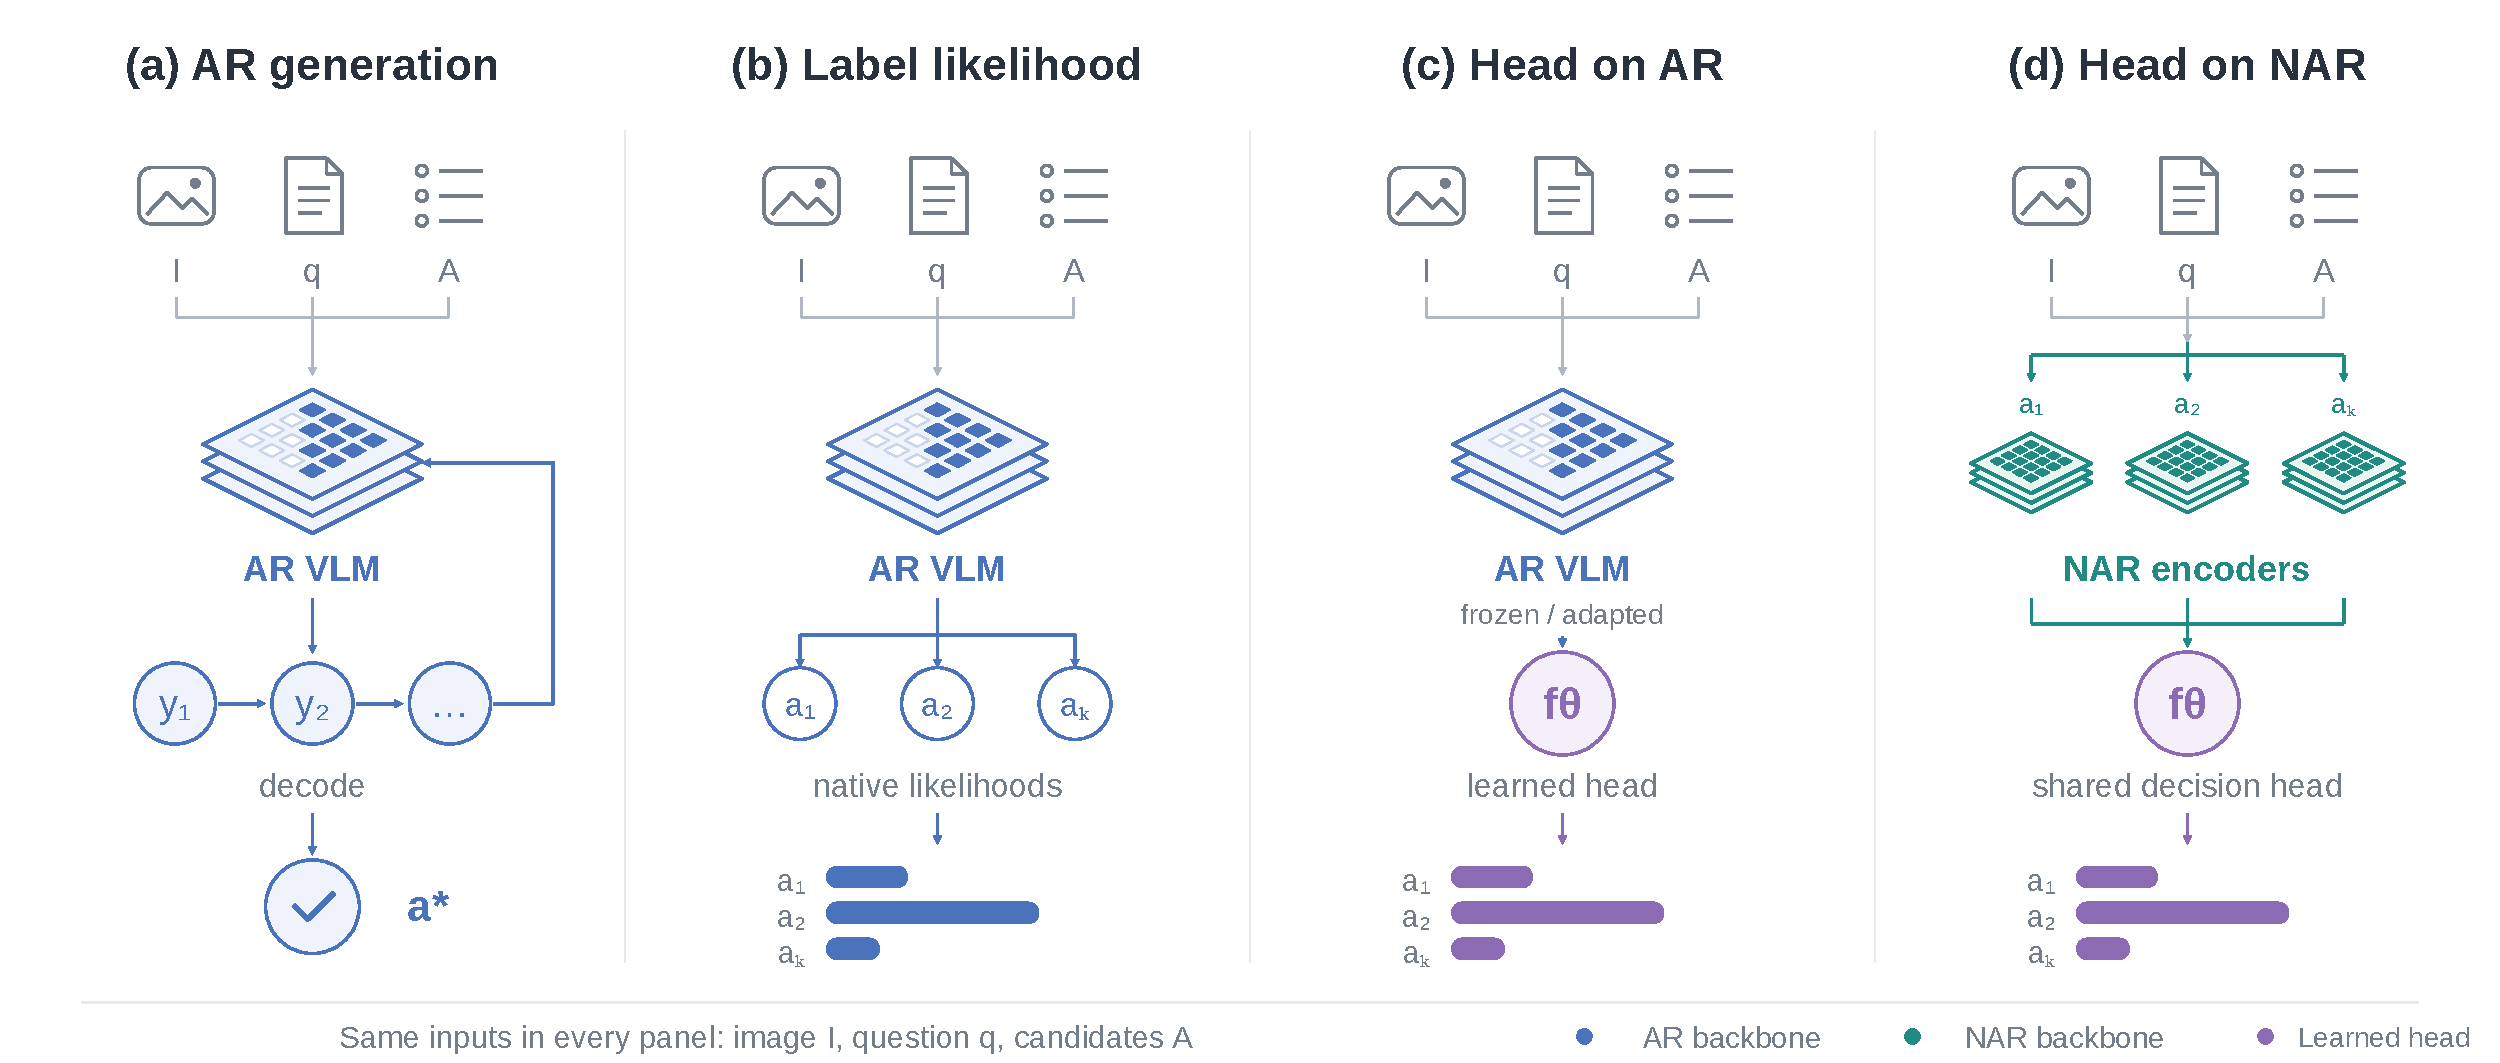
\includegraphics[width=0.50\linewidth]{assets/figures/decision_formulations_refined.pdf}
% \caption{Four bounded-decision formulations: AR-Gen, AR-LL, learned AR interfaces, and NAR-Med.}
% \label{fig:decision_formulations}
% \end{figure}
% 
% \begin{figure}[t]
% \centering
% 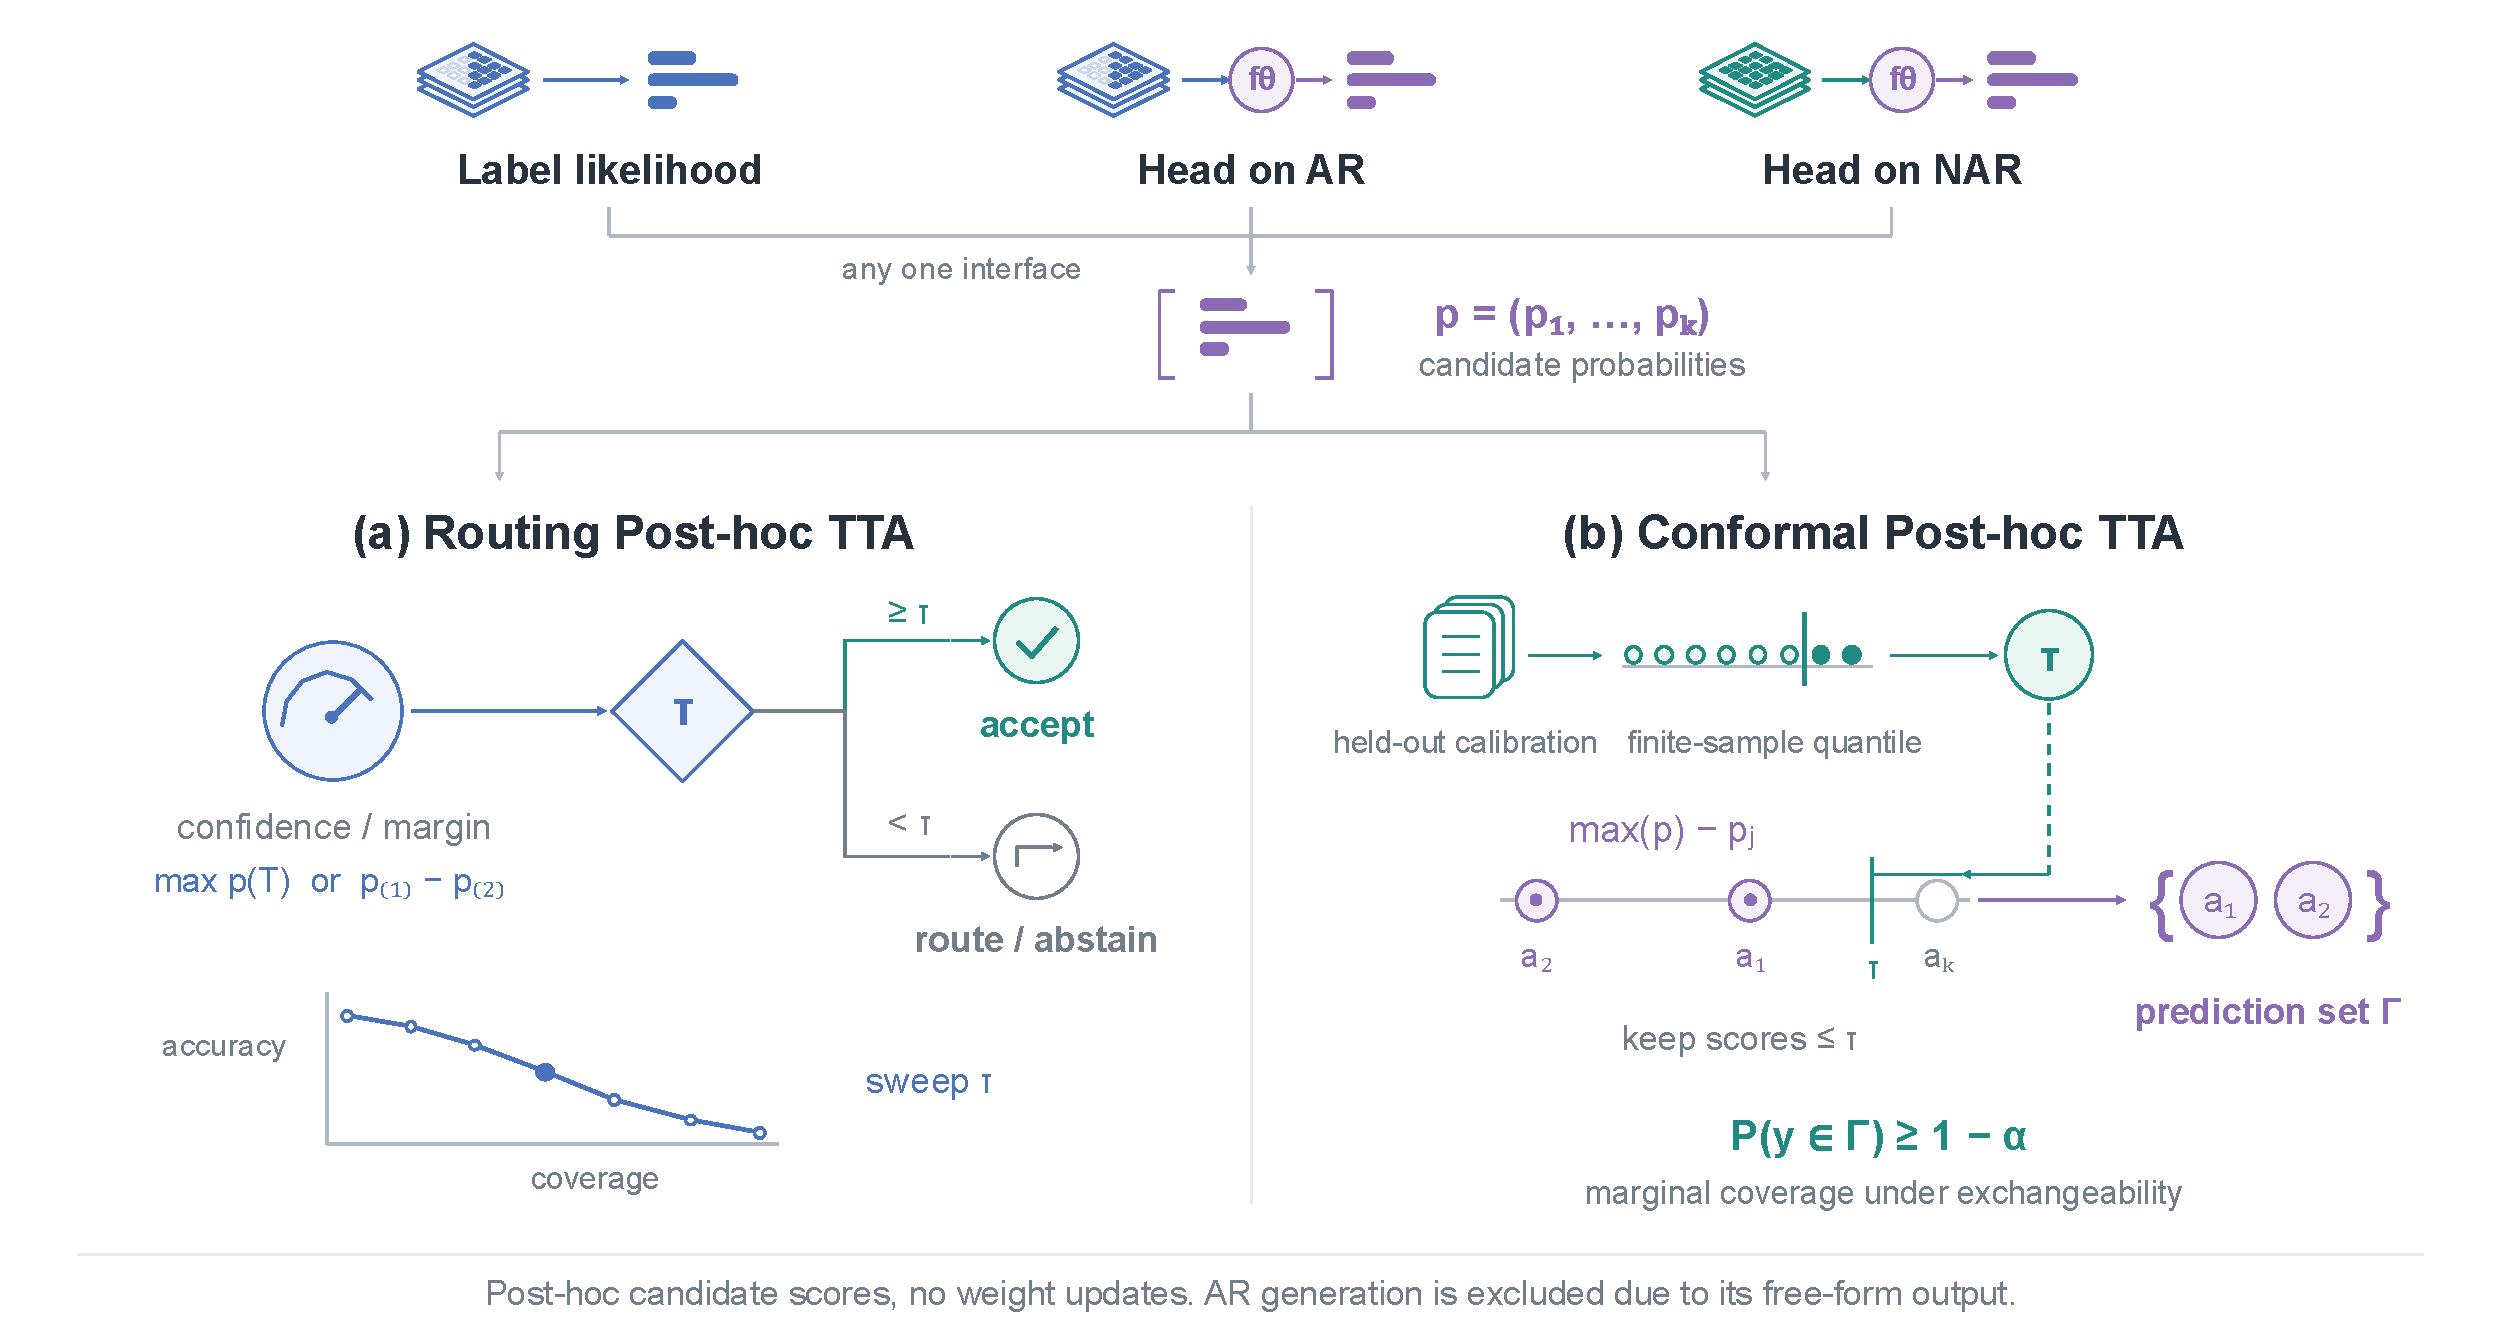
\includegraphics[width=0.50\linewidth]{assets/figures/posthoc_tta_final.pdf}
% \caption{Post-hoc decision policies: confidence routing accepts or defers a prediction; conformal prediction returns a calibrated label set.}
% \label{fig:posthoc_tta_final}
% \end{figure}

\begin{figure*}[t]
\centering

% ============================================================
% LEFT FIGURE
% ============================================================
\begin{minipage}[t]{0.54\textwidth}
    \centering

    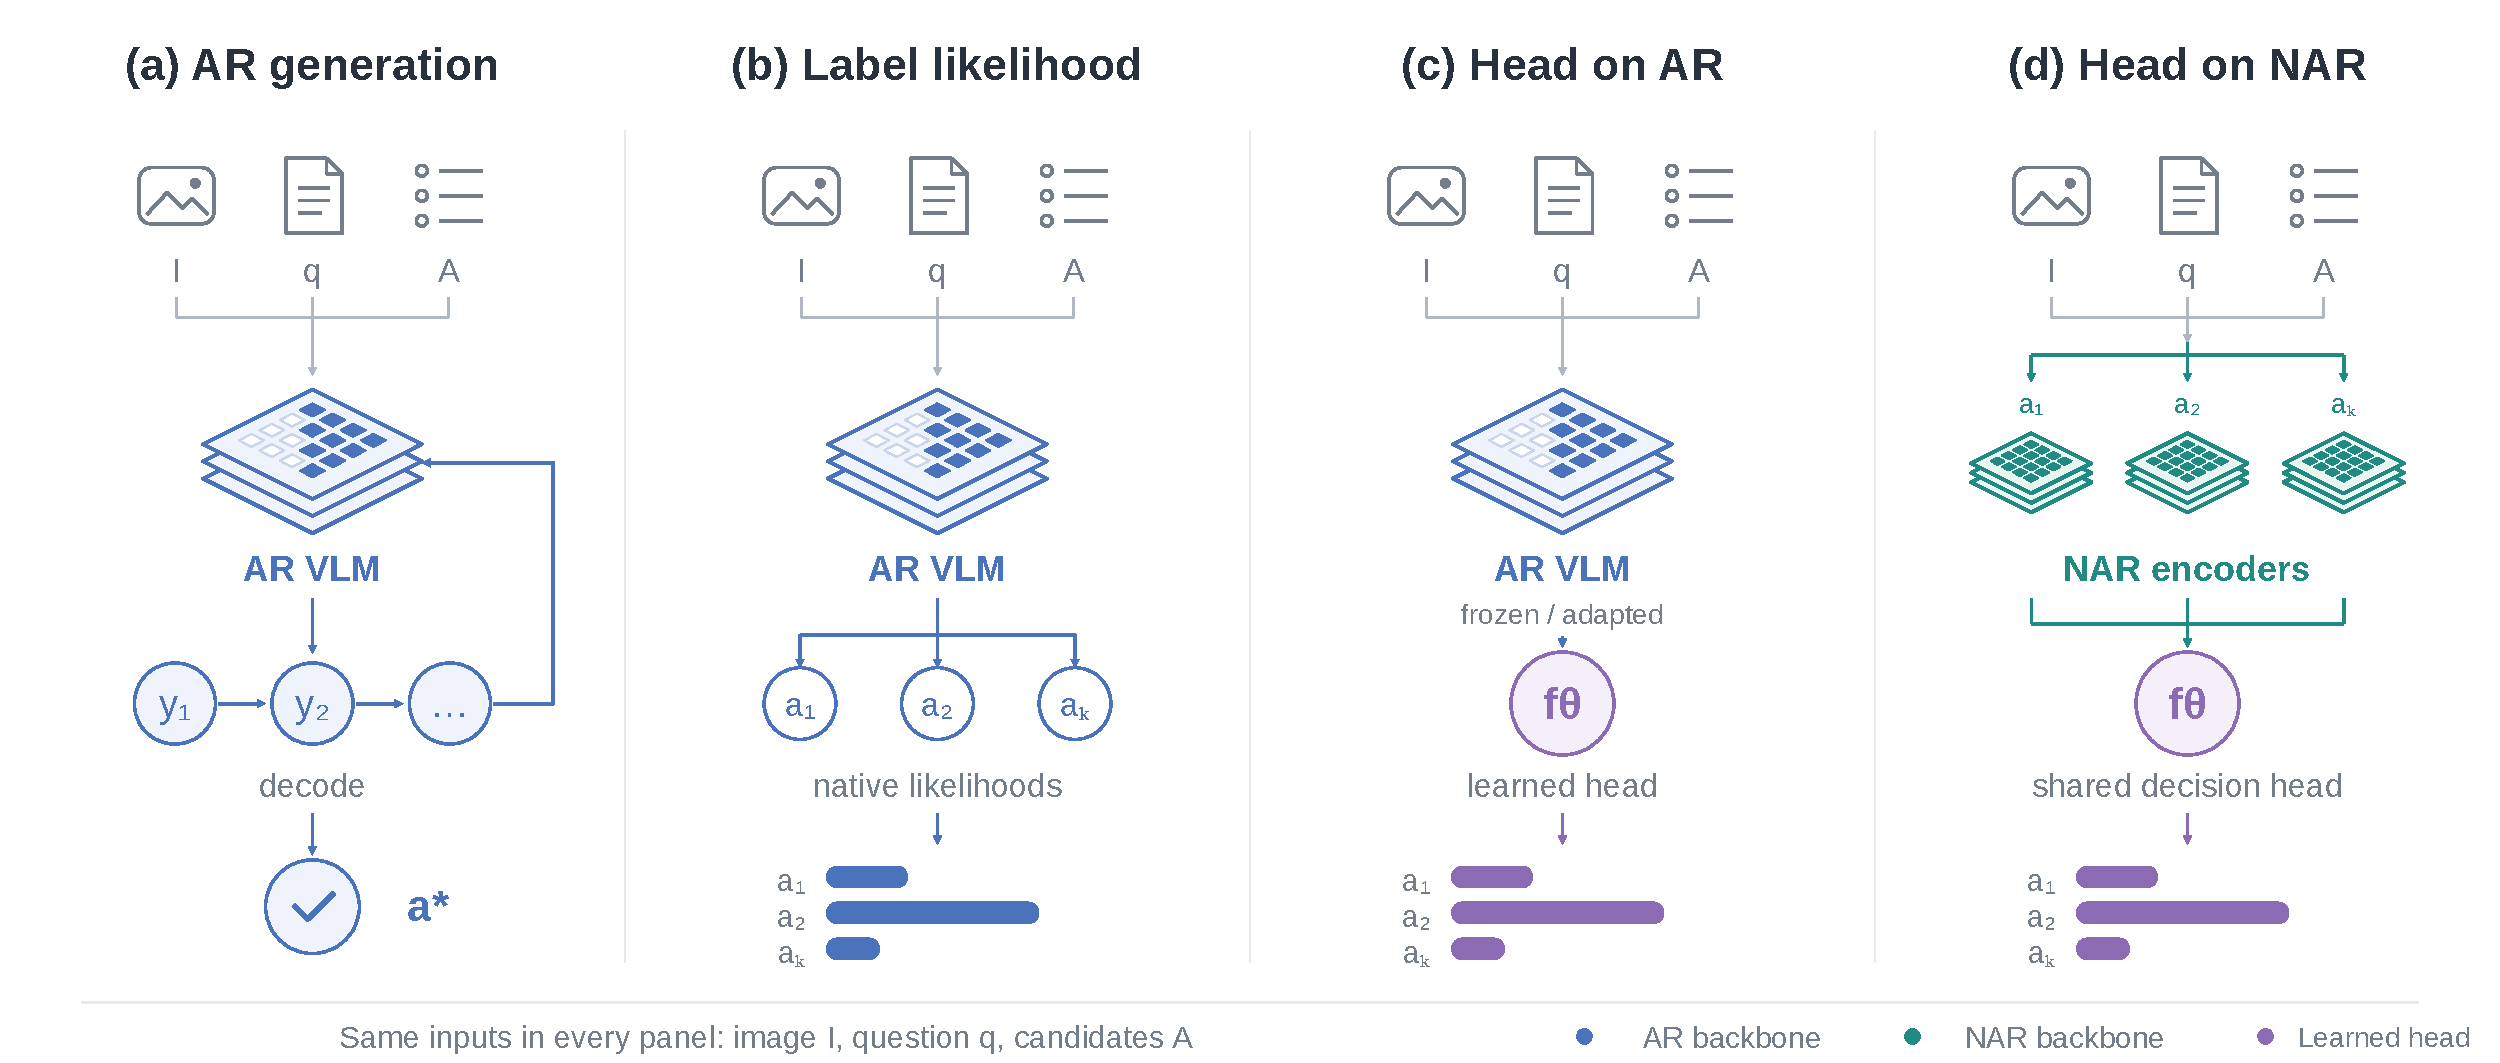
\includegraphics[
        width=\linewidth,
        trim=0 0 0 0,
        clip
    ]{assets/figures/decision_formulations_refined.pdf}

    \captionof{figure}{
    \textbf{Bounded-decision formulations.}
    Four formulations spanning AR-Gen, AR-LL, a learned AR decision
    interface, and a candidate-conditioned NAR decision interface.
    }
    \label{fig:decision_formulations}
\end{minipage}
\hfill
% ============================================================
% RIGHT FIGURE
% ============================================================
\begin{minipage}[t]{0.44\textwidth}
    \centering

    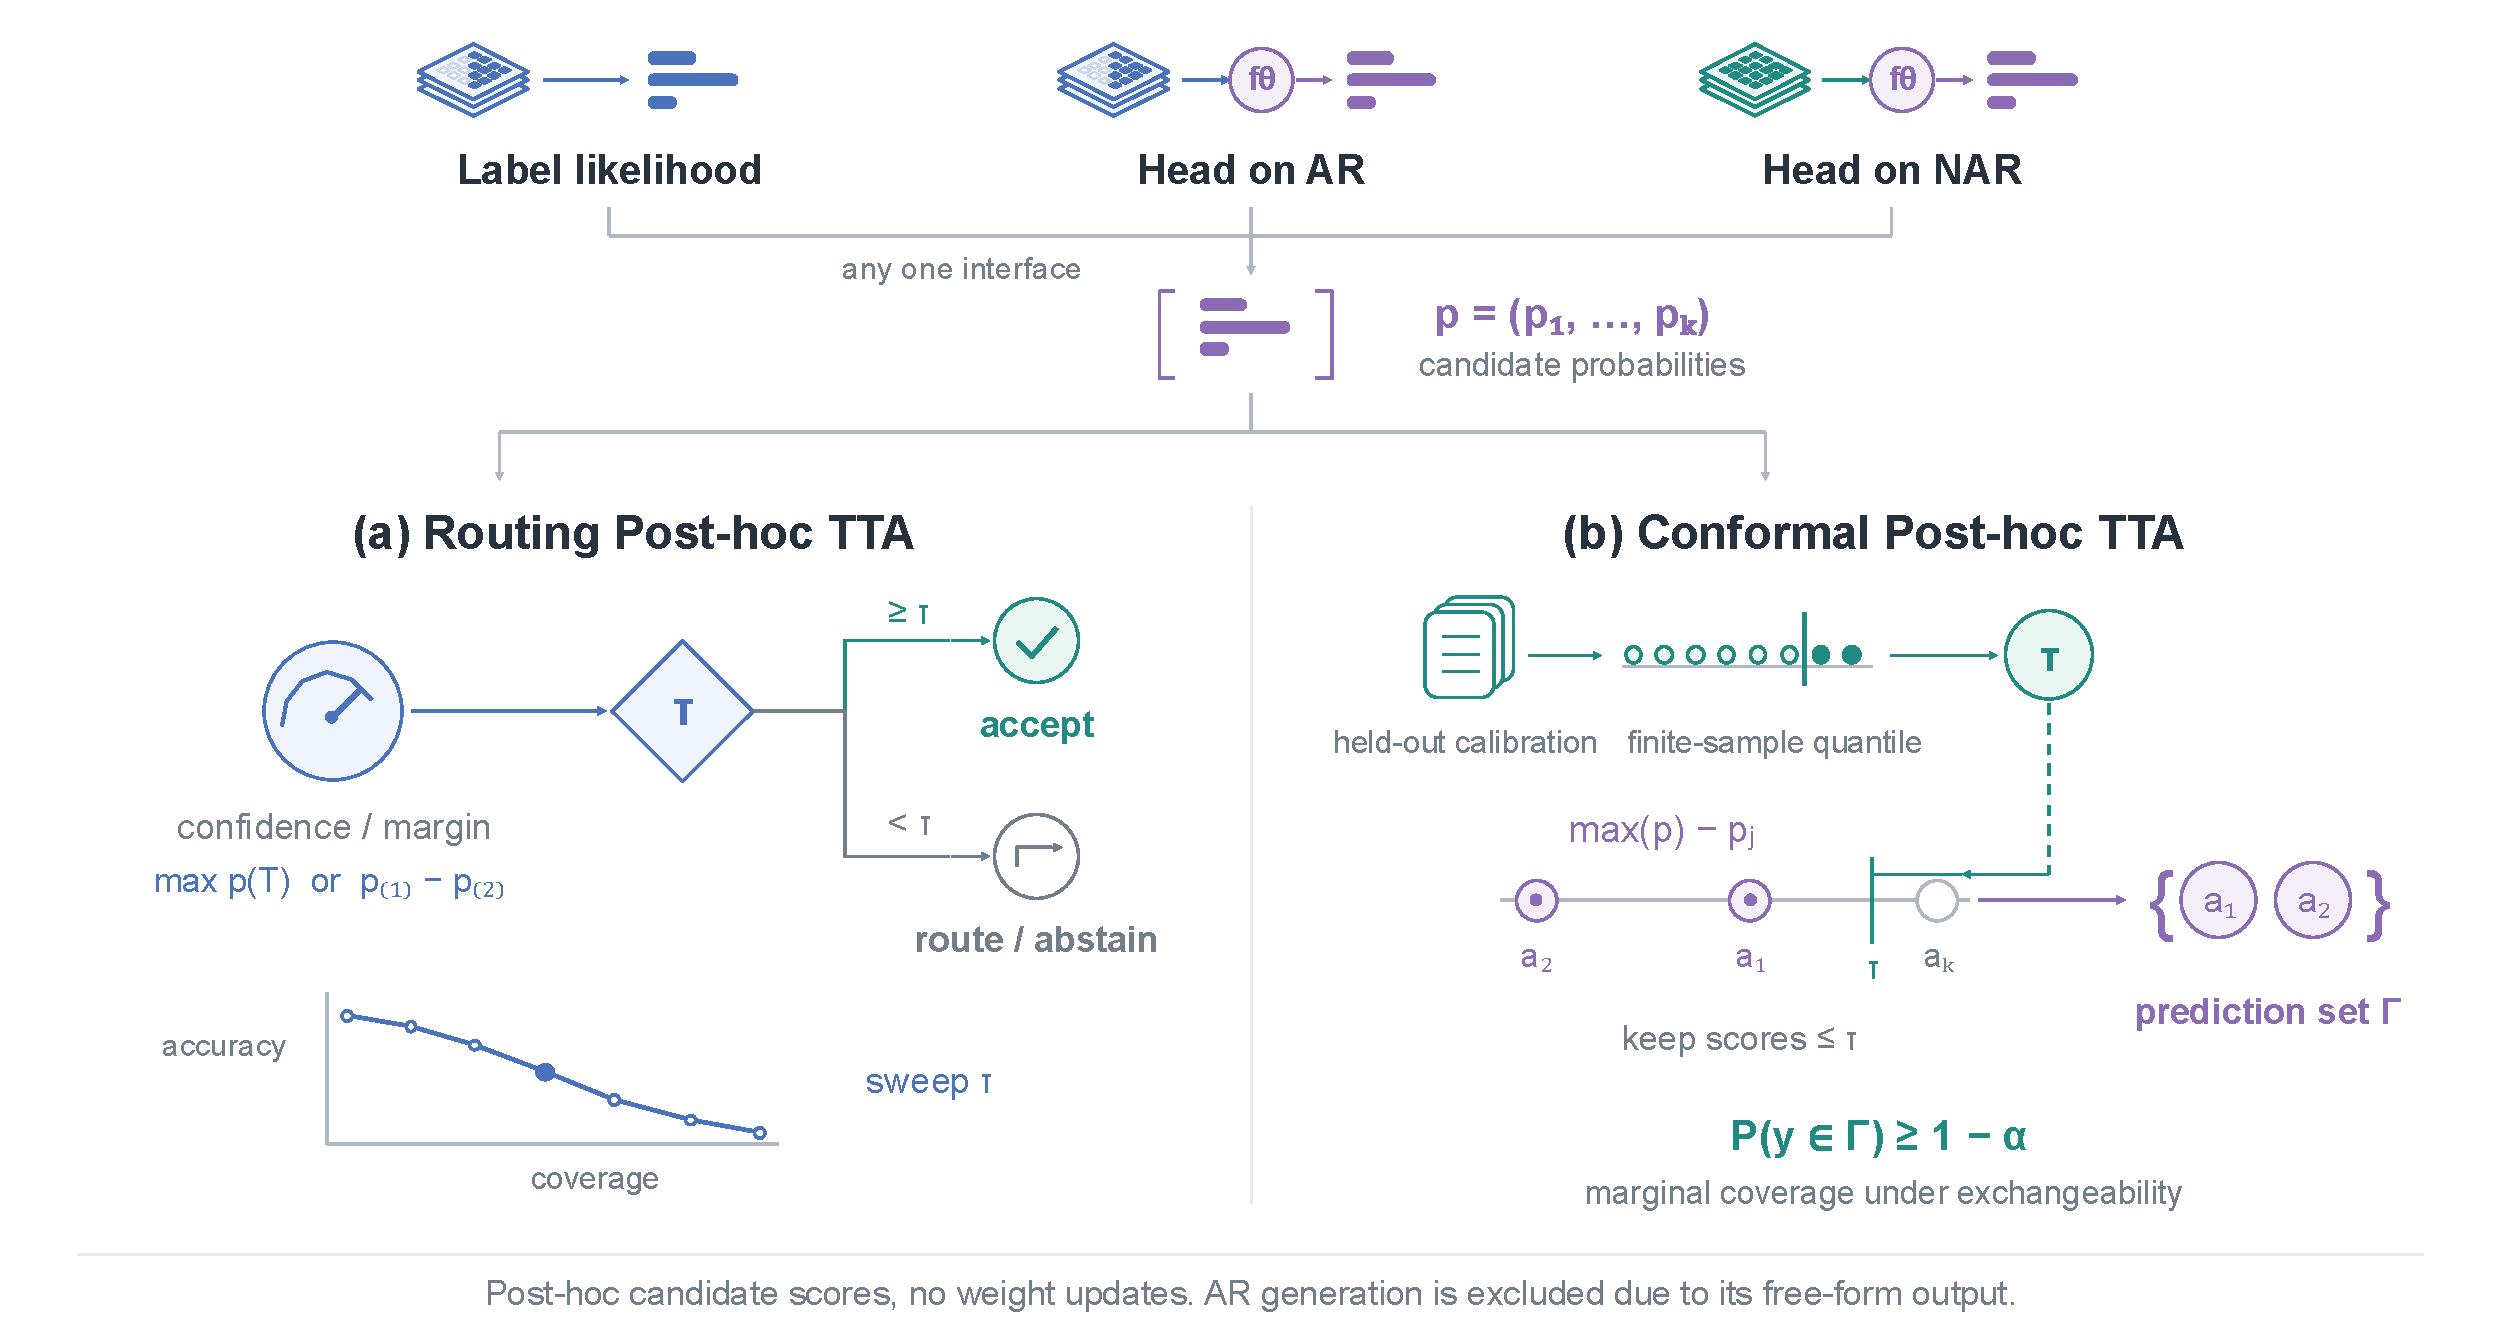
\includegraphics[
        width=\linewidth,
        trim=0 0 0 0,
        clip
    ]{assets/figures/posthoc_tta_final.pdf}

    \captionof{figure}{
    \textbf{Post-hoc decision policies.}
    Confidence routing accepts or defers predictions, while conformal
    prediction constructs calibrated candidate sets.
    }
    \label{fig:posthoc_tta_final}
\end{minipage}

\end{figure*}

\begin{figure*}[t]
\centering
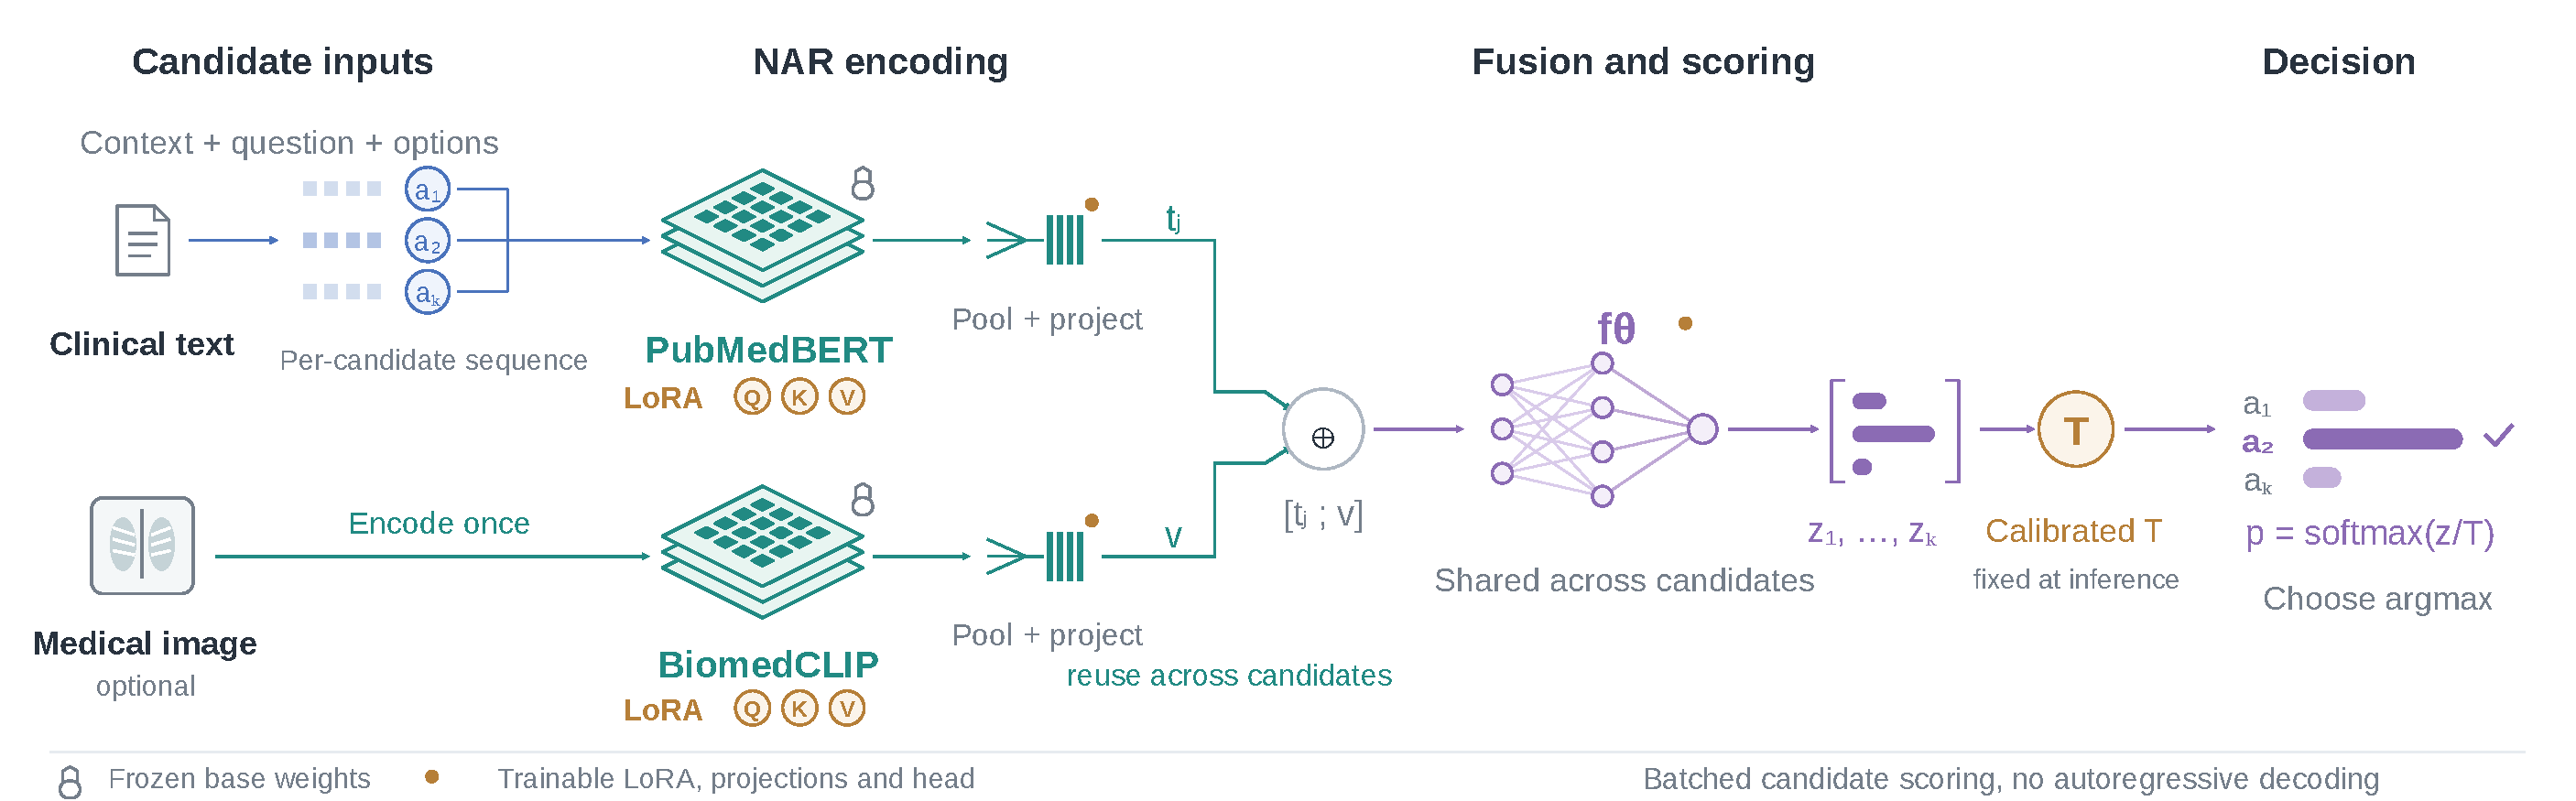
\includegraphics[width=\textwidth]{assets/figures/layamed_multimodal_nar.pdf}
\caption{NAR-Med (Laya-Med) instantiation: candidate-conditioned text features and a shared image representation feed a common decision head.}
\label{fig:main}
\end{figure*}

\subsection{Multimodal Instantiations}
\textbf{Implementation mapping.} MedGemma-4B-IT instantiates AR-Gen, AR-LL, AR-Head, and AR-Adapt. NAR-Med (Laya-Med) uses PubMedBERT and BiomedCLIP encoders; these are distinct backbones, not a matched AR/NAR architecture swap. Jev, MedJev, and NAR (Laya) are external system references (Table~\ref{tab:cohorts}). Formulation names identify decision interfaces; parenthetical model names identify implementations.

\textbf{Learned AR interfaces.} AR-Head caches candidate-specific final hidden states from a frozen MedGemma backbone and trains a 512-dimensional scoring head; AR-Adapt jointly trains that head and rank-8 LoRA adapters on the language-model query, key, value, and output projections, with LoRA scaling $\alpha=16$ and dropout 0.05~\citep{hu2022lora}. AR-Head runs for 15 epochs with batch size 8 and gradient accumulation 8; AR-Adapt runs for 3 epochs with batch size 2 and gradient accumulation 8. Both use learning rate $2\times10^{-4}$, balanced dataset sampling, a 512-token input budget, and seed 42. Training uses AdamW with weight decay 0.01, a cosine schedule with 10\% warmup, and gradient clipping at 1.0. Runs complete the fixed epoch schedule; the checkpoint with highest validation macro accuracy is retained. This contrast fixes the backbone family and candidate interface, but is not training-budget matched; the comparison with AR-LL also changes the supervised objective.

\textbf{Candidate-conditioned NAR interface.} NAR-Med (Laya-Med) fuses candidate-conditioned text features and a shared image feature before a common scoring head (Fig.~\ref{fig:main}). It uses PubMedBERT~\citep{gu2008pubmedbert} and BiomedCLIP~\citep{zhang2023biomedclip}, with rank-8 LoRA adapters on both encoders and a 768-dimensional fusion MLP. Text is encoded for each candidate, while the image representation is computed once and reused. The run uses 15 epochs, batch size 8 with gradient accumulation 4, learning rate $2\times10^{-4}$, balanced dataset sampling, and seed 42; checkpoint selection maximizes validation macro accuracy. Its architecture and optimization differ from the AR systems, so the speed contrast is descriptive of these implementations, not an architecture-only effect.

\textbf{Training, validation, and calibration.} All trained systems use the shared prepared manifest with disjoint train, validation, calibration, and test partitions. Validation selects checkpoints by macro dataset accuracy. NAR-Med runs for 15 epochs with batch size 8 and gradient accumulation 4; its text encoder uses rank-8 LoRA on query/key/value projections, and its vision encoder uses rank-8 LoRA on attention projections. The fusion MLP has hidden dimension 768. It uses the same learning rate, balanced sampling, optimizer, schedule, clipping, and seed as described above. Each run uses one seed (42); example-bootstrap intervals therefore do not measure training-seed variability. After selection, each trained decision model fits one scalar temperature on its separate calibration predictions by minimizing equal-dataset mean NLL over a 121-point log-spaced grid from 0.05 to 20. Temperature is shared across datasets, not fit separately for each dataset. Top-label ECE uses 15 equal-width confidence bins. AR-Gen and AR-LL use their unscaled first-token label-plus-invalid distribution in the probability analysis.

\subsection{Post-hoc Decision Policies}
\label{sec:posthoc-method}
The probability vector exposes uncertainty that can be used after the model is fixed. Fig.~\ref{fig:posthoc_tta_final} illustrates the two policies evaluated here; neither updates the backbone or decision head.

\textbf{Confidence routing.} A prediction is accepted when $\max(p)\geq\tau$ and otherwise deferred. Threshold sweeps describe the trade-off between retained coverage and selective risk; ties at a threshold are retained together. The reference TTA table reports the operating point $\tau=0.7$.

\textbf{Conformal prediction.} We use the score $s(x,y)=\max_j p_j(x)-p_y(x)$ and return $\Gamma(x)=\{i:\max_j p_j(x)-p_i(x)\leq\hat{s}\}$. Only singleton sets yield accepted decisions. In the primary cross-formulation analysis, calibration scores and the finite-sample $\lceil(n+1)(1-\alpha)\rceil$-th order statistic are computed separately for each dataset and method from calibration IDs disjoint from test IDs; if the rank exceeds the calibration set size, the threshold is infinite. This gives marginal, per-dataset coverage under exchangeability, not a guarantee of singleton accuracy. The separate reference TTA table preserves its recorded pooled-quantile operating points for comparability with that source analysis; we do not treat those points as per-dataset validity estimates or as evidence that pooling is preferable. We do not compare alternative nonconformity scores.

\begin{table*}[t]
\centering
\setlength{\tabcolsep}{4pt}
\renewcommand{\arraystretch}{1.13}

\resizebox{\textwidth}{!}{%
\begin{tabular}{@{}lll|lllll@{}}
\toprule
\textbf{Method} &
\textbf{Modality} &
\textbf{Formulation} &
\textbf{Backbone} &
\textbf{Decision} &
\textbf{AR decode?} &
\textbf{Learned head?} &
\textbf{Adaptation} \\
\midrule

AR-Gen
& Text + Image & \textbf{(a)} & AR VLM
& Generation & Yes & No & -- \\

AR-LL
& Text + Image & \textbf{(b)} & AR VLM
& Label likelihood & No & No & None \\

Jev
& Text / structured & \textbf{--}
& Undisclosed & Direct & No & Undisclosed & Proprietary \\

MedJev
& Text only & \textbf{(c)}
& Causal/AR LM & Direct & No & Yes & LoRA + head \\

NAR (Laya)
& Text only & \textbf{(d)}
& NAR encoder & Direct & No & Yes & Decision training \\

\midrule

AR-Head
& Text + Image & \textbf{(c)}
& AR VLM & Direct & No & Yes & Head only \\

AR-Adapt
& Text + Image & \textbf{(c)}
& AR VLM & Direct & No & Yes & LoRA + head \\

NAR-Med (Laya-Med)
& Text + Image & \textbf{(d)}
& NAR encoders & Direct & No & Yes & Decision training \\

\bottomrule
\end{tabular}%
}

\caption{Baseline taxonomy. Formulations \textbf{(a)--(d)} correspond to the design formulations in Fig.~\ref{fig:decision_formulations}. Jev is left unassigned because its internal architecture is undisclosed. The bottom three rows are controlled configurations constructed in this study.}
\label{tab:cohorts}
\end{table*}

\section{Experimental Setup}
\label{sec:setup}

\textbf{Benchmarks and splits.} We evaluate PubMedQA, MedQA, and MedMCQA as text tasks, and VQA-RAD, SLAKE, PathVQA, and PMC-VQA as image tasks. Candidate definitions, labels, and partitions follow one versioned prepared manifest. Preparation groups exact question text and decoded-image duplicates and uses patient/article/group identifiers when supplied; recognized duplicates, conflicting labels, and invalid records are quarantined before splitting. Validation selects checkpoints, calibration fits temperatures and conformal thresholds, and test predictions are reserved for reporting. Saved evaluation runs apply a per-dataset cap; results therefore refer to the prepared test evaluation and should not be described as official full-test results where a prepared split exceeds that cap. MedMCQA and PMC-VQA test partitions are internal holdouts from downloaded training sources, and VQA-RAD uses the prepared group split. These differences constrain comparisons with published official-test results.

\begin{table*}[t]
\centering
\setlength{\tabcolsep}{3.5pt}
\renewcommand{\arraystretch}{1.13}

\resizebox{\textwidth}{!}{%
\begin{tabular}{@{}lllllll@{}}
\toprule
\textbf{Dataset} &
\textbf{Task} &
\textbf{Input} &
\textbf{Domain / Source} &
\textbf{Answer format} &
\textbf{Question type} &
\textbf{Dataset scale} \\
\midrule

PubMedQA
& Biomedical QA
& Text
& PubMed abstracts
& Yes / No / Maybe
& Research reasoning
& 1K expert-labeled \\

MedQA
& Medical MCQA
& Text
& USMLE
& 4 choices
& Clinical / exam
& 12.7K questions \\

MedMCQA
& Medical MCQA
& Text
& AIIMS / NEET-PG
& 4 choices
& Multi-subject exam
& 194K+ questions \\

\midrule

VQA-RAD
& Medical VQA
& Image + Text
& Radiology / MedPix
& Open / closed
& Clinical visual QA
& 315 images / 3.5K QA \\

SLAKE
& Medical VQA
& Image + Text
& CT / MRI / X-ray
& Open / closed
& Visual + knowledge
& 642 images / 14K QA \\

PathVQA
& Medical VQA
& Image + Text
& Pathology
& Open-ended
& Pathology visual QA
& 5.0K images / 32.8K QA \\

PMC-VQA
& Medical VQA
& Image + Text
& Biomedical literature
& Diverse answers
& Biomedical visual QA
& 149K images / 227K QA \\

\bottomrule
\end{tabular}%
}

\caption{
Overview of the seven medical QA and VQA benchmarks used in our study.
The datasets span text-only biomedical and clinical question answering as well
as multimodal reasoning over radiology, pathology, and broader biomedical
imagery.
}
\label{tab:dataset_stats}
\end{table*}

\textbf{Evaluation structure.} The landscape, paired effects, error overlap, confidence--accuracy analysis, visual ablations, and policy curves use the complete set of predictions emitted by their configured evaluation runs. External Jev, MedJev, and NAR (Laya) results provide context, not controlled comparisons, because their model implementations and evaluation pipelines differ. Values from separate runs are not pooled. In the reference policy table, each baseline is recomputed on the same predictions as its corresponding policy.

\textbf{Metrics.} We report accuracy, expected calibration error (ECE), negative log-likelihood (NLL), Brier score, and median latency. Accuracy and probability-quality summaries macro-average datasets unless stated otherwise; pooled paired effects weight examples and need not equal macro differences. For trained heads, ECE is top-label ECE with 15 equal-width bins after scalar temperature scaling. AR-Gen and AR-LL share the same first-token label-plus-invalid probabilities and therefore have identical predictions and probability metrics in this comparison. Paired bootstrap intervals quantify example-sampling uncertainty, not training-seed variability.

\textbf{Policy evaluation.} Accepted accuracy is interpreted together with retained coverage or abstention; it is not a change to full-set accuracy. The reference operating-point table reports routing at $\tau=0.7$ and conformal singleton selection at $\alpha=0.3$. The NAR-Med coverage analysis also reports per-dataset conformal results at $\alpha=0.1$. Cross-formulation risk--coverage curves pool accepted examples within each modality and report routing for AR-LL, AR-Head, AR-Adapt, and NAR-Med. Per-dataset conformal curves are available for AR-Head, AR-Adapt, and NAR-Med, each with separate calibration predictions; AR-LL has no independent calibration export and contributes routing only.

\textbf{Timing and visual dependence.} Timings use synchronized wall-clock measurements, a cold prompt cache, and one warm-up per mode/task; model loading is excluded. AR inference uses batch size 1, the learned MedGemma evaluations use batch size 1, and NAR-Med uses schema-compatible batches up to 8 examples. Precision and implementation boundaries are not fully matched, so these are implementation-level latency comparisons, not a controlled causal speedup claim. Missing-image and shuffled-image ablations compare predictions against their correct-image condition and test image dependence separately from image-task accuracy.

\section{Results}
\label{sec:results}

Table~\ref{tab:sysone-landscape} summarizes the reference accuracy--latency landscape. Rather than treating one average as a verdict, we ask what changes when the decision interface changes, where learning helps, and when confidence supports useful deferral.

\begin{table*}[t]
\centering
\resizebox{\textwidth}{!}{\begin{tikzpicture}[x=1cm,y=1cm,font=\scriptsize]
\node[font=\sffamily\bfseries\small,anchor=west] at (0.100,-0.72) {Task Group};
\node[font=\sffamily\bfseries\small,anchor=west] at (2.630,-0.72) {Dataset};
\fill[gray!9,rounded corners=3pt] (5.050,0) rectangle (6.320,-1.200);
\node[align=center,font=\sffamily\tiny\bfseries] at (5.685,-0.47) {AR-Gen};
\node[align=center,font=\tiny,text=gray!70!black] at (5.685,-0.93) {Acc.\\p50};
\fill[gray!9,rounded corners=3pt] (6.400,0) rectangle (7.670,-1.200);
\node[align=center,font=\sffamily\tiny\bfseries] at (7.035,-0.47) {AR-LL};
\node[align=center,font=\tiny,text=gray!70!black] at (7.035,-0.93) {Acc.\\p50};
\fill[gray!9,rounded corners=3pt] (7.750,0) rectangle (9.020,-1.200);
\node[align=center,font=\sffamily\tiny\bfseries] at (8.385,-0.47) {Jev};
\node[align=center,font=\tiny,text=gray!70!black] at (8.385,-0.93) {Acc.\\p50};
\fill[gray!9,rounded corners=3pt] (9.100,0) rectangle (10.370,-1.200);
\node[align=center,font=\sffamily\tiny\bfseries] at (9.735,-0.47) {MedJev};
\node[align=center,font=\tiny,text=gray!70!black] at (9.735,-0.93) {Acc.\\p50};
\fill[gray!9,rounded corners=3pt] (10.450,0) rectangle (11.720,-1.200);
\node[align=center,font=\sffamily\tiny\bfseries] at (11.085,-0.47) {NAR (Laya)};
\node[align=center,font=\tiny,text=gray!70!black] at (11.085,-0.93) {Acc.\\p50};
\fill[violet!10,rounded corners=3pt] (11.800,0) rectangle (13.070,-1.200);
\node[align=center,font=\sffamily\tiny\bfseries] at (12.435,-0.47) {AR-Head};
\node[align=center,font=\tiny,text=gray!70!black] at (12.435,-0.93) {Acc.\\p50};
\fill[violet!10,rounded corners=3pt] (13.150,0) rectangle (14.420,-1.200);
\node[align=center,font=\sffamily\tiny\bfseries] at (13.785,-0.47) {AR-Adapt};
\node[align=center,font=\tiny,text=gray!70!black] at (13.785,-0.93) {Acc.\\p50};
\fill[violet!10,rounded corners=3pt] (14.500,0) rectangle (15.770,-1.200);
\node[align=center,font=\sffamily\tiny\bfseries] at (15.135,-0.47) {NAR-Med\\(Laya-Med)};
\node[align=center,font=\tiny,text=gray!70!black] at (15.135,-0.93) {Acc.\\p50};
\draw[gray!60,dashed,line width=0.45pt] (11.760,0) -- (11.760,-9.000);
\fill[blue!13,rounded corners=3pt] (0.000,-1.380) rectangle (2.450,-4.300);
\fill[blue!8,rounded corners=3pt] (2.550,-1.380) rectangle (4.900,-4.300);
\node[align=center,text width=2.20cm,font=\sffamily\scriptsize\bfseries,text=blue!55!black] at (1.225,-2.840) {{\Large\faFileMedical}\\[3pt]Text Medical QA};
\node[anchor=west,font=\scriptsize] at (2.670,-1.745) {PubMedQA};
\node[fill={rgb,255:red,218;green,235;blue,185},rounded corners=2pt,minimum width=1.160cm,minimum height=0.270cm,inner sep=0pt,text=black,font=\scriptsize] at (5.685,-1.582) {71.4};
\node[fill={rgb,255:red,248;green,194;blue,187},rounded corners=2pt,minimum width=1.160cm,minimum height=0.270cm,inner sep=0pt,text=gray!65!black,font=\tiny] at (5.685,-1.907) {1034};
\node[fill={rgb,255:red,218;green,235;blue,185},rounded corners=2pt,minimum width=1.160cm,minimum height=0.270cm,inner sep=0pt,text=black,font=\scriptsize] at (7.035,-1.582) {71.4};
\node[fill={rgb,255:red,147;green,214;blue,175},rounded corners=2pt,minimum width=1.160cm,minimum height=0.270cm,inner sep=0pt,text=gray!65!black,font=\tiny] at (7.035,-1.907) {51};
\node[fill={rgb,255:red,139;green,211;blue,174},rounded corners=2pt,minimum width=1.160cm,minimum height=0.270cm,inner sep=0pt,text=black,font=\scriptsize] at (8.385,-1.582) {\textbf{78.8}};
\node[fill={rgb,255:red,246;green,232;blue,183},rounded corners=2pt,minimum width=1.160cm,minimum height=0.270cm,inner sep=0pt,text=gray!65!black,font=\tiny] at (8.385,-1.907) {587};
\node[fill={rgb,255:red,250;green,223;blue,181},rounded corners=2pt,minimum width=1.160cm,minimum height=0.270cm,inner sep=0pt,text=black,font=\scriptsize] at (9.735,-1.582) {63.8};
\node[fill={rgb,255:red,157;green,217;blue,177},rounded corners=2pt,minimum width=1.160cm,minimum height=0.270cm,inner sep=0pt,text=gray!65!black,font=\tiny] at (9.735,-1.907) {90};
\node[fill={rgb,255:red,248;green,194;blue,187},rounded corners=2pt,minimum width=1.160cm,minimum height=0.270cm,inner sep=0pt,text=black,font=\scriptsize] at (11.085,-1.582) {56.6};
\node[fill={rgb,255:red,139;green,211;blue,174},rounded corners=2pt,minimum width=1.160cm,minimum height=0.270cm,inner sep=0pt,text=gray!65!black,font=\tiny] at (11.085,-1.907) {\textbf{19}};
\node[fill={rgb,255:red,247;green,229;blue,182},rounded corners=2pt,minimum width=1.160cm,minimum height=0.270cm,inner sep=0pt,text=black,font=\scriptsize] at (12.435,-1.582) {65.6};
\node[fill={rgb,255:red,183;green,226;blue,181},rounded corners=2pt,minimum width=1.160cm,minimum height=0.270cm,inner sep=0pt,text=gray!65!black,font=\tiny] at (12.435,-1.907) {198};
\node[fill={rgb,255:red,206;green,232;blue,184},rounded corners=2pt,minimum width=1.160cm,minimum height=0.270cm,inner sep=0pt,text=black,font=\scriptsize] at (13.785,-1.582) {72.6};
\node[fill={rgb,255:red,186;green,226;blue,182},rounded corners=2pt,minimum width=1.160cm,minimum height=0.270cm,inner sep=0pt,text=gray!65!black,font=\tiny] at (13.785,-1.907) {210};
\node[fill={rgb,255:red,250;green,224;blue,181},rounded corners=2pt,minimum width=1.160cm,minimum height=0.270cm,inner sep=0pt,text=black,font=\scriptsize] at (15.135,-1.582) {64.0};
\node[fill={rgb,255:red,140;green,211;blue,174},rounded corners=2pt,minimum width=1.160cm,minimum height=0.270cm,inner sep=0pt,text=gray!65!black,font=\tiny] at (15.135,-1.907) {24};
\node[anchor=west,font=\scriptsize] at (2.670,-2.475) {MedQA};
\node[fill={rgb,255:red,246;green,231;blue,183},rounded corners=2pt,minimum width=1.160cm,minimum height=0.270cm,inner sep=0pt,text=black,font=\scriptsize] at (5.685,-2.312) {49.2};
\node[fill={rgb,255:red,248;green,194;blue,187},rounded corners=2pt,minimum width=1.160cm,minimum height=0.270cm,inner sep=0pt,text=gray!65!black,font=\tiny] at (5.685,-2.637) {1065};
\node[fill={rgb,255:red,246;green,231;blue,183},rounded corners=2pt,minimum width=1.160cm,minimum height=0.270cm,inner sep=0pt,text=black,font=\scriptsize] at (7.035,-2.312) {49.2};
\node[fill={rgb,255:red,147;green,214;blue,175},rounded corners=2pt,minimum width=1.160cm,minimum height=0.270cm,inner sep=0pt,text=gray!65!black,font=\tiny] at (7.035,-2.637) {51};
\node[fill={rgb,255:red,139;green,211;blue,174},rounded corners=2pt,minimum width=1.160cm,minimum height=0.270cm,inner sep=0pt,text=black,font=\scriptsize] at (8.385,-2.312) {\textbf{86.1}};
\node[fill={rgb,255:red,245;green,233;blue,183},rounded corners=2pt,minimum width=1.160cm,minimum height=0.270cm,inner sep=0pt,text=gray!65!black,font=\tiny] at (8.385,-2.637) {584};
\node[fill={rgb,255:red,249;green,203;blue,184},rounded corners=2pt,minimum width=1.160cm,minimum height=0.270cm,inner sep=0pt,text=black,font=\scriptsize] at (9.735,-2.312) {28.3};
\node[fill={rgb,255:red,155;green,216;blue,177},rounded corners=2pt,minimum width=1.160cm,minimum height=0.270cm,inner sep=0pt,text=gray!65!black,font=\tiny] at (9.735,-2.637) {85};
\node[fill={rgb,255:red,248;green,194;blue,187},rounded corners=2pt,minimum width=1.160cm,minimum height=0.270cm,inner sep=0pt,text=black,font=\scriptsize] at (11.085,-2.312) {21.1};
\node[fill={rgb,255:red,139;green,211;blue,174},rounded corners=2pt,minimum width=1.160cm,minimum height=0.270cm,inner sep=0pt,text=gray!65!black,font=\tiny] at (11.085,-2.637) {\textbf{18}};
\node[fill={rgb,255:red,245;green,234;blue,183},rounded corners=2pt,minimum width=1.160cm,minimum height=0.270cm,inner sep=0pt,text=black,font=\scriptsize] at (12.435,-2.312) {51.5};
\node[fill={rgb,255:red,187;green,227;blue,182},rounded corners=2pt,minimum width=1.160cm,minimum height=0.270cm,inner sep=0pt,text=gray!65!black,font=\tiny] at (12.435,-2.637) {221};
\node[fill={rgb,255:red,244;green,236;blue,184},rounded corners=2pt,minimum width=1.160cm,minimum height=0.270cm,inner sep=0pt,text=black,font=\scriptsize] at (13.785,-2.312) {53.3};
\node[fill={rgb,255:red,191;green,228;blue,182},rounded corners=2pt,minimum width=1.160cm,minimum height=0.270cm,inner sep=0pt,text=gray!65!black,font=\tiny] at (13.785,-2.637) {239};
\node[fill={rgb,255:red,249;green,205;blue,184},rounded corners=2pt,minimum width=1.160cm,minimum height=0.270cm,inner sep=0pt,text=black,font=\scriptsize] at (15.135,-2.312) {30.4};
\node[fill={rgb,255:red,142;green,212;blue,175},rounded corners=2pt,minimum width=1.160cm,minimum height=0.270cm,inner sep=0pt,text=gray!65!black,font=\tiny] at (15.135,-2.637) {32};
\node[anchor=west,font=\scriptsize] at (2.670,-3.205) {MedMCQA};
\node[fill={rgb,255:red,234;green,236;blue,184},rounded corners=2pt,minimum width=1.160cm,minimum height=0.270cm,inner sep=0pt,text=black,font=\scriptsize] at (5.685,-3.042) {60.2};
\node[fill={rgb,255:red,248;green,194;blue,187},rounded corners=2pt,minimum width=1.160cm,minimum height=0.270cm,inner sep=0pt,text=gray!65!black,font=\tiny] at (5.685,-3.368) {1049};
\node[fill={rgb,255:red,234;green,236;blue,184},rounded corners=2pt,minimum width=1.160cm,minimum height=0.270cm,inner sep=0pt,text=black,font=\scriptsize] at (7.035,-3.042) {60.2};
\node[fill={rgb,255:red,146;green,213;blue,175},rounded corners=2pt,minimum width=1.160cm,minimum height=0.270cm,inner sep=0pt,text=gray!65!black,font=\tiny] at (7.035,-3.368) {35};
\node[fill={rgb,255:red,139;green,211;blue,174},rounded corners=2pt,minimum width=1.160cm,minimum height=0.270cm,inner sep=0pt,text=black,font=\scriptsize] at (8.385,-3.042) {\textbf{85.0}};
\node[fill={rgb,255:red,246;green,232;blue,183},rounded corners=2pt,minimum width=1.160cm,minimum height=0.270cm,inner sep=0pt,text=gray!65!black,font=\tiny] at (8.385,-3.368) {587};
\node[fill={rgb,255:red,249;green,205;blue,184},rounded corners=2pt,minimum width=1.160cm,minimum height=0.270cm,inner sep=0pt,text=black,font=\scriptsize] at (9.735,-3.042) {35.9};
\node[fill={rgb,255:red,156;green,217;blue,177},rounded corners=2pt,minimum width=1.160cm,minimum height=0.270cm,inner sep=0pt,text=gray!65!black,font=\tiny] at (9.735,-3.368) {75};
\node[fill={rgb,255:red,248;green,194;blue,187},rounded corners=2pt,minimum width=1.160cm,minimum height=0.270cm,inner sep=0pt,text=black,font=\scriptsize] at (11.085,-3.042) {27.7};
\node[fill={rgb,255:red,142;green,212;blue,174},rounded corners=2pt,minimum width=1.160cm,minimum height=0.270cm,inner sep=0pt,text=gray!65!black,font=\tiny] at (11.085,-3.368) {18};
\node[fill={rgb,255:red,219;green,235;blue,185},rounded corners=2pt,minimum width=1.160cm,minimum height=0.270cm,inner sep=0pt,text=black,font=\scriptsize] at (12.435,-3.042) {65.5};
\node[fill={rgb,255:red,154;green,216;blue,177},rounded corners=2pt,minimum width=1.160cm,minimum height=0.270cm,inner sep=0pt,text=gray!65!black,font=\tiny] at (12.435,-3.368) {70};
\node[fill={rgb,255:red,207;green,232;blue,184},rounded corners=2pt,minimum width=1.160cm,minimum height=0.270cm,inner sep=0pt,text=black,font=\scriptsize] at (13.785,-3.042) {68.7};
\node[fill={rgb,255:red,156;green,217;blue,177},rounded corners=2pt,minimum width=1.160cm,minimum height=0.270cm,inner sep=0pt,text=gray!65!black,font=\tiny] at (13.785,-3.368) {77};
\node[fill={rgb,255:red,249;green,213;blue,182},rounded corners=2pt,minimum width=1.160cm,minimum height=0.270cm,inner sep=0pt,text=black,font=\scriptsize] at (15.135,-3.042) {40.8};
\node[fill={rgb,255:red,139;green,211;blue,174},rounded corners=2pt,minimum width=1.160cm,minimum height=0.270cm,inner sep=0pt,text=gray!65!black,font=\tiny] at (15.135,-3.368) {\textbf{6}};
\node[anchor=west,font=\scriptsize] at (2.670,-3.935) {\textbf{Text Average}};
\node[fill={rgb,255:red,241;green,236;blue,184},rounded corners=2pt,minimum width=1.160cm,minimum height=0.270cm,inner sep=0pt,text=black,font=\scriptsize] at (5.685,-3.772) {60.3};
\node[fill={rgb,255:red,248;green,194;blue,187},rounded corners=2pt,minimum width=1.160cm,minimum height=0.270cm,inner sep=0pt,text=gray!65!black,font=\tiny] at (5.685,-4.097) {1050};
\node[fill={rgb,255:red,241;green,236;blue,184},rounded corners=2pt,minimum width=1.160cm,minimum height=0.270cm,inner sep=0pt,text=black,font=\scriptsize] at (7.035,-3.772) {60.3};
\node[fill={rgb,255:red,146;green,213;blue,175},rounded corners=2pt,minimum width=1.160cm,minimum height=0.270cm,inner sep=0pt,text=gray!65!black,font=\tiny] at (7.035,-4.097) {46};
\node[fill={rgb,255:red,139;green,211;blue,174},rounded corners=2pt,minimum width=1.160cm,minimum height=0.270cm,inner sep=0pt,text=black,font=\scriptsize] at (8.385,-3.772) {\textbf{83.3}};
\node[fill={rgb,255:red,246;green,232;blue,183},rounded corners=2pt,minimum width=1.160cm,minimum height=0.270cm,inner sep=0pt,text=gray!65!black,font=\tiny] at (8.385,-4.097) {586};
\node[fill={rgb,255:red,249;green,206;blue,183},rounded corners=2pt,minimum width=1.160cm,minimum height=0.270cm,inner sep=0pt,text=black,font=\scriptsize] at (9.735,-3.772) {42.7};
\node[fill={rgb,255:red,155;green,216;blue,177},rounded corners=2pt,minimum width=1.160cm,minimum height=0.270cm,inner sep=0pt,text=gray!65!black,font=\tiny] at (9.735,-4.097) {83};
\node[fill={rgb,255:red,248;green,194;blue,187},rounded corners=2pt,minimum width=1.160cm,minimum height=0.270cm,inner sep=0pt,text=black,font=\scriptsize] at (11.085,-3.772) {35.1};
\node[fill={rgb,255:red,139;green,211;blue,174},rounded corners=2pt,minimum width=1.160cm,minimum height=0.270cm,inner sep=0pt,text=gray!65!black,font=\tiny] at (11.085,-4.097) {\textbf{18}};
\node[fill={rgb,255:red,239;green,236;blue,184},rounded corners=2pt,minimum width=1.160cm,minimum height=0.270cm,inner sep=0pt,text=black,font=\scriptsize] at (12.435,-3.772) {60.8};
\node[fill={rgb,255:red,174;green,223;blue,180},rounded corners=2pt,minimum width=1.160cm,minimum height=0.270cm,inner sep=0pt,text=gray!65!black,font=\tiny] at (12.435,-4.097) {163};
\node[fill={rgb,255:red,226;green,235;blue,185},rounded corners=2pt,minimum width=1.160cm,minimum height=0.270cm,inner sep=0pt,text=black,font=\scriptsize] at (13.785,-3.772) {64.9};
\node[fill={rgb,255:red,177;green,224;blue,180},rounded corners=2pt,minimum width=1.160cm,minimum height=0.270cm,inner sep=0pt,text=gray!65!black,font=\tiny] at (13.785,-4.097) {175};
\node[fill={rgb,255:red,249;green,211;blue,183},rounded corners=2pt,minimum width=1.160cm,minimum height=0.270cm,inner sep=0pt,text=black,font=\scriptsize] at (15.135,-3.772) {45.1};
\node[fill={rgb,255:red,140;green,211;blue,174},rounded corners=2pt,minimum width=1.160cm,minimum height=0.270cm,inner sep=0pt,text=gray!65!black,font=\tiny] at (15.135,-4.097) {21};
\draw[gray!40,line width=0.35pt] (2.550,-3.570) -- (15.770,-3.570);
\fill[teal!13,rounded corners=3pt] (0.000,-4.460) rectangle (2.450,-8.110);
\fill[teal!8,rounded corners=3pt] (2.550,-4.460) rectangle (4.900,-8.110);
\node[align=center,text width=2.20cm,font=\sffamily\scriptsize\bfseries,text=teal!55!black] at (1.225,-6.285) {{\Large\faMicroscope}\\[3pt]Medical VQA};
\node[anchor=west,font=\scriptsize] at (2.670,-4.825) {VQA-RAD};
\node[fill={rgb,255:red,205;green,231;blue,184},rounded corners=2pt,minimum width=1.160cm,minimum height=0.270cm,inner sep=0pt,text=black,font=\scriptsize] at (5.685,-4.663) {70.6};
\node[fill={rgb,255:red,248;green,194;blue,187},rounded corners=2pt,minimum width=1.160cm,minimum height=0.270cm,inner sep=0pt,text=gray!65!black,font=\tiny] at (5.685,-4.987) {1168};
\node[fill={rgb,255:red,205;green,231;blue,184},rounded corners=2pt,minimum width=1.160cm,minimum height=0.270cm,inner sep=0pt,text=black,font=\scriptsize] at (7.035,-4.663) {70.6};
\node[fill={rgb,255:red,170;green,221;blue,179},rounded corners=2pt,minimum width=1.160cm,minimum height=0.270cm,inner sep=0pt,text=gray!65!black,font=\tiny] at (7.035,-4.987) {148};
\node[fill=gray!12,rounded corners=2pt,minimum width=1.160cm,minimum height=0.270cm,inner sep=0pt,text=gray!55] at (8.385,-4.663) {n/s};
\node[fill=gray!12,rounded corners=2pt,minimum width=1.160cm,minimum height=0.270cm,inner sep=0pt,text=gray!55] at (8.385,-4.987) {n/s};
\node[fill=gray!12,rounded corners=2pt,minimum width=1.160cm,minimum height=0.270cm,inner sep=0pt,text=gray!55] at (9.735,-4.663) {n/s};
\node[fill=gray!12,rounded corners=2pt,minimum width=1.160cm,minimum height=0.270cm,inner sep=0pt,text=gray!55] at (9.735,-4.987) {n/s};
\node[fill=gray!12,rounded corners=2pt,minimum width=1.160cm,minimum height=0.270cm,inner sep=0pt,text=gray!55] at (11.085,-4.663) {n/s};
\node[fill=gray!12,rounded corners=2pt,minimum width=1.160cm,minimum height=0.270cm,inner sep=0pt,text=gray!55] at (11.085,-4.987) {n/s};
\node[fill={rgb,255:red,139;green,211;blue,174},rounded corners=2pt,minimum width=1.160cm,minimum height=0.270cm,inner sep=0pt,text=black,font=\scriptsize] at (12.435,-4.663) {\textbf{76.1}};
\node[fill={rgb,255:red,214;green,234;blue,185},rounded corners=2pt,minimum width=1.160cm,minimum height=0.270cm,inner sep=0pt,text=gray!65!black,font=\tiny] at (12.435,-4.987) {373};
\node[fill={rgb,255:red,215;green,234;blue,185},rounded corners=2pt,minimum width=1.160cm,minimum height=0.270cm,inner sep=0pt,text=black,font=\scriptsize] at (13.785,-4.663) {69.7};
\node[fill={rgb,255:red,215;green,234;blue,185},rounded corners=2pt,minimum width=1.160cm,minimum height=0.270cm,inner sep=0pt,text=gray!65!black,font=\tiny] at (13.785,-4.987) {376};
\node[fill={rgb,255:red,248;green,194;blue,187},rounded corners=2pt,minimum width=1.160cm,minimum height=0.270cm,inner sep=0pt,text=black,font=\scriptsize] at (15.135,-4.663) {56.0};
\node[fill={rgb,255:red,139;green,211;blue,174},rounded corners=2pt,minimum width=1.160cm,minimum height=0.270cm,inner sep=0pt,text=gray!65!black,font=\tiny] at (15.135,-4.987) {\textbf{5}};
\node[anchor=west,font=\scriptsize] at (2.670,-5.555) {SLAKE};
\node[fill={rgb,255:red,248;green,194;blue,187},rounded corners=2pt,minimum width=1.160cm,minimum height=0.270cm,inner sep=0pt,text=black,font=\scriptsize] at (5.685,-5.393) {79.4};
\node[fill={rgb,255:red,248;green,194;blue,187},rounded corners=2pt,minimum width=1.160cm,minimum height=0.270cm,inner sep=0pt,text=gray!65!black,font=\tiny] at (5.685,-5.717) {1159};
\node[fill={rgb,255:red,248;green,194;blue,187},rounded corners=2pt,minimum width=1.160cm,minimum height=0.270cm,inner sep=0pt,text=black,font=\scriptsize] at (7.035,-5.393) {79.4};
\node[fill={rgb,255:red,170;green,221;blue,179},rounded corners=2pt,minimum width=1.160cm,minimum height=0.270cm,inner sep=0pt,text=gray!65!black,font=\tiny] at (7.035,-5.717) {152};
\node[fill=gray!12,rounded corners=2pt,minimum width=1.160cm,minimum height=0.270cm,inner sep=0pt,text=gray!55] at (8.385,-5.393) {n/s};
\node[fill=gray!12,rounded corners=2pt,minimum width=1.160cm,minimum height=0.270cm,inner sep=0pt,text=gray!55] at (8.385,-5.717) {n/s};
\node[fill=gray!12,rounded corners=2pt,minimum width=1.160cm,minimum height=0.270cm,inner sep=0pt,text=gray!55] at (9.735,-5.393) {n/s};
\node[fill=gray!12,rounded corners=2pt,minimum width=1.160cm,minimum height=0.270cm,inner sep=0pt,text=gray!55] at (9.735,-5.717) {n/s};
\node[fill=gray!12,rounded corners=2pt,minimum width=1.160cm,minimum height=0.270cm,inner sep=0pt,text=gray!55] at (11.085,-5.393) {n/s};
\node[fill=gray!12,rounded corners=2pt,minimum width=1.160cm,minimum height=0.270cm,inner sep=0pt,text=gray!55] at (11.085,-5.717) {n/s};
\node[fill={rgb,255:red,221;green,235;blue,185},rounded corners=2pt,minimum width=1.160cm,minimum height=0.270cm,inner sep=0pt,text=black,font=\scriptsize] at (12.435,-5.393) {86.8};
\node[fill={rgb,255:red,215;green,234;blue,185},rounded corners=2pt,minimum width=1.160cm,minimum height=0.270cm,inner sep=0pt,text=gray!65!black,font=\tiny] at (12.435,-5.717) {376};
\node[fill={rgb,255:red,139;green,211;blue,174},rounded corners=2pt,minimum width=1.160cm,minimum height=0.270cm,inner sep=0pt,text=black,font=\scriptsize] at (13.785,-5.393) {\textbf{90.7}};
\node[fill={rgb,255:red,217;green,235;blue,185},rounded corners=2pt,minimum width=1.160cm,minimum height=0.270cm,inner sep=0pt,text=gray!65!black,font=\tiny] at (13.785,-5.717) {385};
\node[fill={rgb,255:red,248;green,198;blue,186},rounded corners=2pt,minimum width=1.160cm,minimum height=0.270cm,inner sep=0pt,text=black,font=\scriptsize] at (15.135,-5.393) {80.0};
\node[fill={rgb,255:red,139;green,211;blue,174},rounded corners=2pt,minimum width=1.160cm,minimum height=0.270cm,inner sep=0pt,text=gray!65!black,font=\tiny] at (15.135,-5.717) {\textbf{9}};
\node[anchor=west,font=\scriptsize] at (2.670,-6.285) {PathVQA};
\node[fill={rgb,255:red,248;green,194;blue,187},rounded corners=2pt,minimum width=1.160cm,minimum height=0.270cm,inner sep=0pt,text=black,font=\scriptsize] at (5.685,-6.123) {62.3};
\node[fill={rgb,255:red,248;green,194;blue,187},rounded corners=2pt,minimum width=1.160cm,minimum height=0.270cm,inner sep=0pt,text=gray!65!black,font=\tiny] at (5.685,-6.447) {1162};
\node[fill={rgb,255:red,248;green,194;blue,187},rounded corners=2pt,minimum width=1.160cm,minimum height=0.270cm,inner sep=0pt,text=black,font=\scriptsize] at (7.035,-6.123) {62.3};
\node[fill={rgb,255:red,171;green,222;blue,179},rounded corners=2pt,minimum width=1.160cm,minimum height=0.270cm,inner sep=0pt,text=gray!65!black,font=\tiny] at (7.035,-6.447) {153};
\node[fill=gray!12,rounded corners=2pt,minimum width=1.160cm,minimum height=0.270cm,inner sep=0pt,text=gray!55] at (8.385,-6.123) {n/s};
\node[fill=gray!12,rounded corners=2pt,minimum width=1.160cm,minimum height=0.270cm,inner sep=0pt,text=gray!55] at (8.385,-6.447) {n/s};
\node[fill=gray!12,rounded corners=2pt,minimum width=1.160cm,minimum height=0.270cm,inner sep=0pt,text=gray!55] at (9.735,-6.123) {n/s};
\node[fill=gray!12,rounded corners=2pt,minimum width=1.160cm,minimum height=0.270cm,inner sep=0pt,text=gray!55] at (9.735,-6.447) {n/s};
\node[fill=gray!12,rounded corners=2pt,minimum width=1.160cm,minimum height=0.270cm,inner sep=0pt,text=gray!55] at (11.085,-6.123) {n/s};
\node[fill=gray!12,rounded corners=2pt,minimum width=1.160cm,minimum height=0.270cm,inner sep=0pt,text=gray!55] at (11.085,-6.447) {n/s};
\node[fill={rgb,255:red,173;green,222;blue,180},rounded corners=2pt,minimum width=1.160cm,minimum height=0.270cm,inner sep=0pt,text=black,font=\scriptsize] at (12.435,-6.123) {86.3};
\node[fill={rgb,255:red,215;green,234;blue,185},rounded corners=2pt,minimum width=1.160cm,minimum height=0.270cm,inner sep=0pt,text=gray!65!black,font=\tiny] at (12.435,-6.447) {378};
\node[fill={rgb,255:red,139;green,211;blue,174},rounded corners=2pt,minimum width=1.160cm,minimum height=0.270cm,inner sep=0pt,text=black,font=\scriptsize] at (13.785,-6.123) {\textbf{90.0}};
\node[fill={rgb,255:red,216;green,234;blue,185},rounded corners=2pt,minimum width=1.160cm,minimum height=0.270cm,inner sep=0pt,text=gray!65!black,font=\tiny] at (13.785,-6.447) {381};
\node[fill={rgb,255:red,168;green,221;blue,179},rounded corners=2pt,minimum width=1.160cm,minimum height=0.270cm,inner sep=0pt,text=black,font=\scriptsize] at (15.135,-6.123) {86.9};
\node[fill={rgb,255:red,139;green,211;blue,174},rounded corners=2pt,minimum width=1.160cm,minimum height=0.270cm,inner sep=0pt,text=gray!65!black,font=\tiny] at (15.135,-6.447) {\textbf{5}};
\node[anchor=west,font=\scriptsize] at (2.670,-7.015) {PMC-VQA};
\node[fill={rgb,255:red,250;green,219;blue,182},rounded corners=2pt,minimum width=1.160cm,minimum height=0.270cm,inner sep=0pt,text=black,font=\scriptsize] at (5.685,-6.853) {48.7};
\node[fill={rgb,255:red,248;green,194;blue,187},rounded corners=2pt,minimum width=1.160cm,minimum height=0.270cm,inner sep=0pt,text=gray!65!black,font=\tiny] at (5.685,-7.178) {1160};
\node[fill={rgb,255:red,250;green,219;blue,182},rounded corners=2pt,minimum width=1.160cm,minimum height=0.270cm,inner sep=0pt,text=black,font=\scriptsize] at (7.035,-6.853) {48.7};
\node[fill={rgb,255:red,169;green,221;blue,179},rounded corners=2pt,minimum width=1.160cm,minimum height=0.270cm,inner sep=0pt,text=gray!65!black,font=\tiny] at (7.035,-7.178) {147};
\node[fill=gray!12,rounded corners=2pt,minimum width=1.160cm,minimum height=0.270cm,inner sep=0pt,text=gray!55] at (8.385,-6.853) {n/s};
\node[fill=gray!12,rounded corners=2pt,minimum width=1.160cm,minimum height=0.270cm,inner sep=0pt,text=gray!55] at (8.385,-7.178) {n/s};
\node[fill=gray!12,rounded corners=2pt,minimum width=1.160cm,minimum height=0.270cm,inner sep=0pt,text=gray!55] at (9.735,-6.853) {n/s};
\node[fill=gray!12,rounded corners=2pt,minimum width=1.160cm,minimum height=0.270cm,inner sep=0pt,text=gray!55] at (9.735,-7.178) {n/s};
\node[fill=gray!12,rounded corners=2pt,minimum width=1.160cm,minimum height=0.270cm,inner sep=0pt,text=gray!55] at (11.085,-6.853) {n/s};
\node[fill=gray!12,rounded corners=2pt,minimum width=1.160cm,minimum height=0.270cm,inner sep=0pt,text=gray!55] at (11.085,-7.178) {n/s};
\node[fill={rgb,255:red,142;green,212;blue,175},rounded corners=2pt,minimum width=1.160cm,minimum height=0.270cm,inner sep=0pt,text=black,font=\scriptsize] at (12.435,-6.853) {57.1};
\node[fill={rgb,255:red,248;green,228;blue,182},rounded corners=2pt,minimum width=1.160cm,minimum height=0.270cm,inner sep=0pt,text=gray!65!black,font=\tiny] at (12.435,-7.178) {719};
\node[fill={rgb,255:red,139;green,211;blue,174},rounded corners=2pt,minimum width=1.160cm,minimum height=0.270cm,inner sep=0pt,text=black,font=\scriptsize] at (13.785,-6.853) {\textbf{57.2}};
\node[fill={rgb,255:red,248;green,228;blue,182},rounded corners=2pt,minimum width=1.160cm,minimum height=0.270cm,inner sep=0pt,text=gray!65!black,font=\tiny] at (13.785,-7.178) {714};
\node[fill={rgb,255:red,248;green,194;blue,187},rounded corners=2pt,minimum width=1.160cm,minimum height=0.270cm,inner sep=0pt,text=black,font=\scriptsize] at (15.135,-6.853) {45.4};
\node[fill={rgb,255:red,139;green,211;blue,174},rounded corners=2pt,minimum width=1.160cm,minimum height=0.270cm,inner sep=0pt,text=gray!65!black,font=\tiny] at (15.135,-7.178) {\textbf{9}};
\node[anchor=west,font=\scriptsize] at (2.670,-7.745) {\textbf{Image Average}};
\node[fill={rgb,255:red,248;green,194;blue,187},rounded corners=2pt,minimum width=1.160cm,minimum height=0.270cm,inner sep=0pt,text=black,font=\scriptsize] at (5.685,-7.583) {65.3};
\node[fill={rgb,255:red,248;green,194;blue,187},rounded corners=2pt,minimum width=1.160cm,minimum height=0.270cm,inner sep=0pt,text=gray!65!black,font=\tiny] at (5.685,-7.908) {1162};
\node[fill={rgb,255:red,248;green,194;blue,187},rounded corners=2pt,minimum width=1.160cm,minimum height=0.270cm,inner sep=0pt,text=black,font=\scriptsize] at (7.035,-7.583) {65.3};
\node[fill={rgb,255:red,170;green,221;blue,179},rounded corners=2pt,minimum width=1.160cm,minimum height=0.270cm,inner sep=0pt,text=gray!65!black,font=\tiny] at (7.035,-7.908) {150};
\node[fill=gray!12,rounded corners=2pt,minimum width=1.160cm,minimum height=0.270cm,inner sep=0pt,text=gray!55] at (8.385,-7.583) {n/s};
\node[fill=gray!12,rounded corners=2pt,minimum width=1.160cm,minimum height=0.270cm,inner sep=0pt,text=gray!55] at (8.385,-7.908) {n/s};
\node[fill=gray!12,rounded corners=2pt,minimum width=1.160cm,minimum height=0.270cm,inner sep=0pt,text=gray!55] at (9.735,-7.583) {n/s};
\node[fill=gray!12,rounded corners=2pt,minimum width=1.160cm,minimum height=0.270cm,inner sep=0pt,text=gray!55] at (9.735,-7.908) {n/s};
\node[fill=gray!12,rounded corners=2pt,minimum width=1.160cm,minimum height=0.270cm,inner sep=0pt,text=gray!55] at (11.085,-7.583) {n/s};
\node[fill=gray!12,rounded corners=2pt,minimum width=1.160cm,minimum height=0.270cm,inner sep=0pt,text=gray!55] at (11.085,-7.908) {n/s};
\node[fill={rgb,255:red,147;green,214;blue,175},rounded corners=2pt,minimum width=1.160cm,minimum height=0.270cm,inner sep=0pt,text=black,font=\scriptsize] at (12.435,-7.583) {76.6};
\node[fill={rgb,255:red,227;green,235;blue,185},rounded corners=2pt,minimum width=1.160cm,minimum height=0.270cm,inner sep=0pt,text=gray!65!black,font=\tiny] at (12.435,-7.908) {461};
\node[fill={rgb,255:red,139;green,211;blue,174},rounded corners=2pt,minimum width=1.160cm,minimum height=0.270cm,inner sep=0pt,text=black,font=\scriptsize] at (13.785,-7.583) {\textbf{76.9}};
\node[fill={rgb,255:red,228;green,235;blue,185},rounded corners=2pt,minimum width=1.160cm,minimum height=0.270cm,inner sep=0pt,text=gray!65!black,font=\tiny] at (13.785,-7.908) {464};
\node[fill={rgb,255:red,249;green,206;blue,183},rounded corners=2pt,minimum width=1.160cm,minimum height=0.270cm,inner sep=0pt,text=black,font=\scriptsize] at (15.135,-7.583) {67.0};
\node[fill={rgb,255:red,139;green,211;blue,174},rounded corners=2pt,minimum width=1.160cm,minimum height=0.270cm,inner sep=0pt,text=gray!65!black,font=\tiny] at (15.135,-7.908) {\textbf{7}};
\draw[gray!40,line width=0.35pt] (2.550,-7.380) -- (15.770,-7.380);
\fill[violet!13,rounded corners=3pt] (0.000,-8.270) rectangle (2.450,-9.000);
\fill[violet!8,rounded corners=3pt] (2.550,-8.270) rectangle (4.900,-9.000);
\node[align=center,text width=2.20cm,font=\sffamily\scriptsize\bfseries,text=violet!55!black] at (1.225,-8.635) {Overall};
\node[anchor=west,font=\scriptsize] at (2.670,-8.635) {\textbf{Overall Average}};
\node[fill={rgb,255:red,231;green,236;blue,184},rounded corners=2pt,minimum width=1.160cm,minimum height=0.270cm,inner sep=0pt,text=black,font=\scriptsize] at (5.685,-8.473) {63.1};
\node[fill={rgb,255:red,248;green,194;blue,187},rounded corners=2pt,minimum width=1.160cm,minimum height=0.270cm,inner sep=0pt,text=gray!65!black,font=\tiny] at (5.685,-8.798) {1114};
\node[fill={rgb,255:red,231;green,236;blue,184},rounded corners=2pt,minimum width=1.160cm,minimum height=0.270cm,inner sep=0pt,text=black,font=\scriptsize] at (7.035,-8.473) {63.1};
\node[fill={rgb,255:red,160;green,218;blue,178},rounded corners=2pt,minimum width=1.160cm,minimum height=0.270cm,inner sep=0pt,text=gray!65!black,font=\tiny] at (7.035,-8.798) {105};
\node[fill={rgb,255:red,139;green,211;blue,174},rounded corners=2pt,minimum width=1.160cm,minimum height=0.270cm,inner sep=0pt,text=black,font=\scriptsize] at (8.385,-8.473) {\textbf{83.3}};
\node[fill={rgb,255:red,245;green,235;blue,184},rounded corners=2pt,minimum width=1.160cm,minimum height=0.270cm,inner sep=0pt,text=gray!65!black,font=\tiny] at (8.385,-8.798) {586};
\node[fill={rgb,255:red,249;green,206;blue,183},rounded corners=2pt,minimum width=1.160cm,minimum height=0.270cm,inner sep=0pt,text=black,font=\scriptsize] at (9.735,-8.473) {42.7};
\node[fill={rgb,255:red,155;green,216;blue,177},rounded corners=2pt,minimum width=1.160cm,minimum height=0.270cm,inner sep=0pt,text=gray!65!black,font=\tiny] at (9.735,-8.798) {83};
\node[fill={rgb,255:red,248;green,194;blue,187},rounded corners=2pt,minimum width=1.160cm,minimum height=0.270cm,inner sep=0pt,text=black,font=\scriptsize] at (11.085,-8.473) {35.1};
\node[fill={rgb,255:red,140;green,211;blue,174},rounded corners=2pt,minimum width=1.160cm,minimum height=0.270cm,inner sep=0pt,text=gray!65!black,font=\tiny] at (11.085,-8.798) {18};
\node[fill={rgb,255:red,206;green,232;blue,184},rounded corners=2pt,minimum width=1.160cm,minimum height=0.270cm,inner sep=0pt,text=black,font=\scriptsize] at (12.435,-8.473) {69.8};
\node[fill={rgb,255:red,209;green,232;blue,184},rounded corners=2pt,minimum width=1.160cm,minimum height=0.270cm,inner sep=0pt,text=gray!65!black,font=\tiny] at (12.435,-8.798) {334};
\node[fill={rgb,255:red,197;green,229;blue,183},rounded corners=2pt,minimum width=1.160cm,minimum height=0.270cm,inner sep=0pt,text=black,font=\scriptsize] at (13.785,-8.473) {71.8};
\node[fill={rgb,255:red,210;green,233;blue,184},rounded corners=2pt,minimum width=1.160cm,minimum height=0.270cm,inner sep=0pt,text=gray!65!black,font=\tiny] at (13.785,-8.798) {340};
\node[fill={rgb,255:red,245;green,234;blue,183},rounded corners=2pt,minimum width=1.160cm,minimum height=0.270cm,inner sep=0pt,text=black,font=\scriptsize] at (15.135,-8.473) {57.6};
\node[fill={rgb,255:red,139;green,211;blue,174},rounded corners=2pt,minimum width=1.160cm,minimum height=0.270cm,inner sep=0pt,text=gray!65!black,font=\tiny] at (15.135,-8.798) {\textbf{13}};
\draw[gray!40,line width=0.35pt] (2.550,-8.270) -- (15.770,-8.270);
\node[font=\tiny\itshape,text=gray!70!black] at (13.785,0.18) {Controlled configurations};
\node[anchor=west,font=\sffamily\scriptsize] at (3.500,-9.550) {Worst};
\fill[fill={rgb,255:red,248;green,194;blue,187},rounded corners=1.5pt] (4.550,-9.700) rectangle (4.970,-9.400);
\fill[fill={rgb,255:red,249;green,207;blue,183},rounded corners=1.5pt] (5.050,-9.700) rectangle (5.470,-9.400);
\fill[fill={rgb,255:red,250;green,224;blue,181},rounded corners=1.5pt] (5.550,-9.700) rectangle (5.970,-9.400);
\fill[fill={rgb,255:red,244;green,236;blue,184},rounded corners=1.5pt] (6.050,-9.700) rectangle (6.470,-9.400);
\fill[fill={rgb,255:red,218;green,235;blue,185},rounded corners=1.5pt] (6.550,-9.700) rectangle (6.970,-9.400);
\fill[fill={rgb,255:red,181;green,225;blue,181},rounded corners=1.5pt] (7.050,-9.700) rectangle (7.470,-9.400);
\fill[fill={rgb,255:red,139;green,211;blue,174},rounded corners=1.5pt] (7.550,-9.700) rectangle (7.970,-9.400);
\node[anchor=west,font=\sffamily\scriptsize] at (8.100,-9.550) {Best};
\node[fill=gray!12,rounded corners=2pt,minimum width=0.48cm,minimum height=0.30cm,inner sep=0pt,text=gray!55] at (10.950,-9.550) {n/s};
\node[anchor=west,font=\sffamily\scriptsize,text=black] at (11.330,-9.550) {not supported};
\end{tikzpicture}}
\caption{Accuracy--latency landscape for the predictions in the configured test evaluations. Cells show accuracy (top) and median latency in milliseconds (bottom); bold marks the best available value per row and metric.}
\label{tab:sysone-landscape}
\end{table*}

\begin{figure*}[t]
\centering
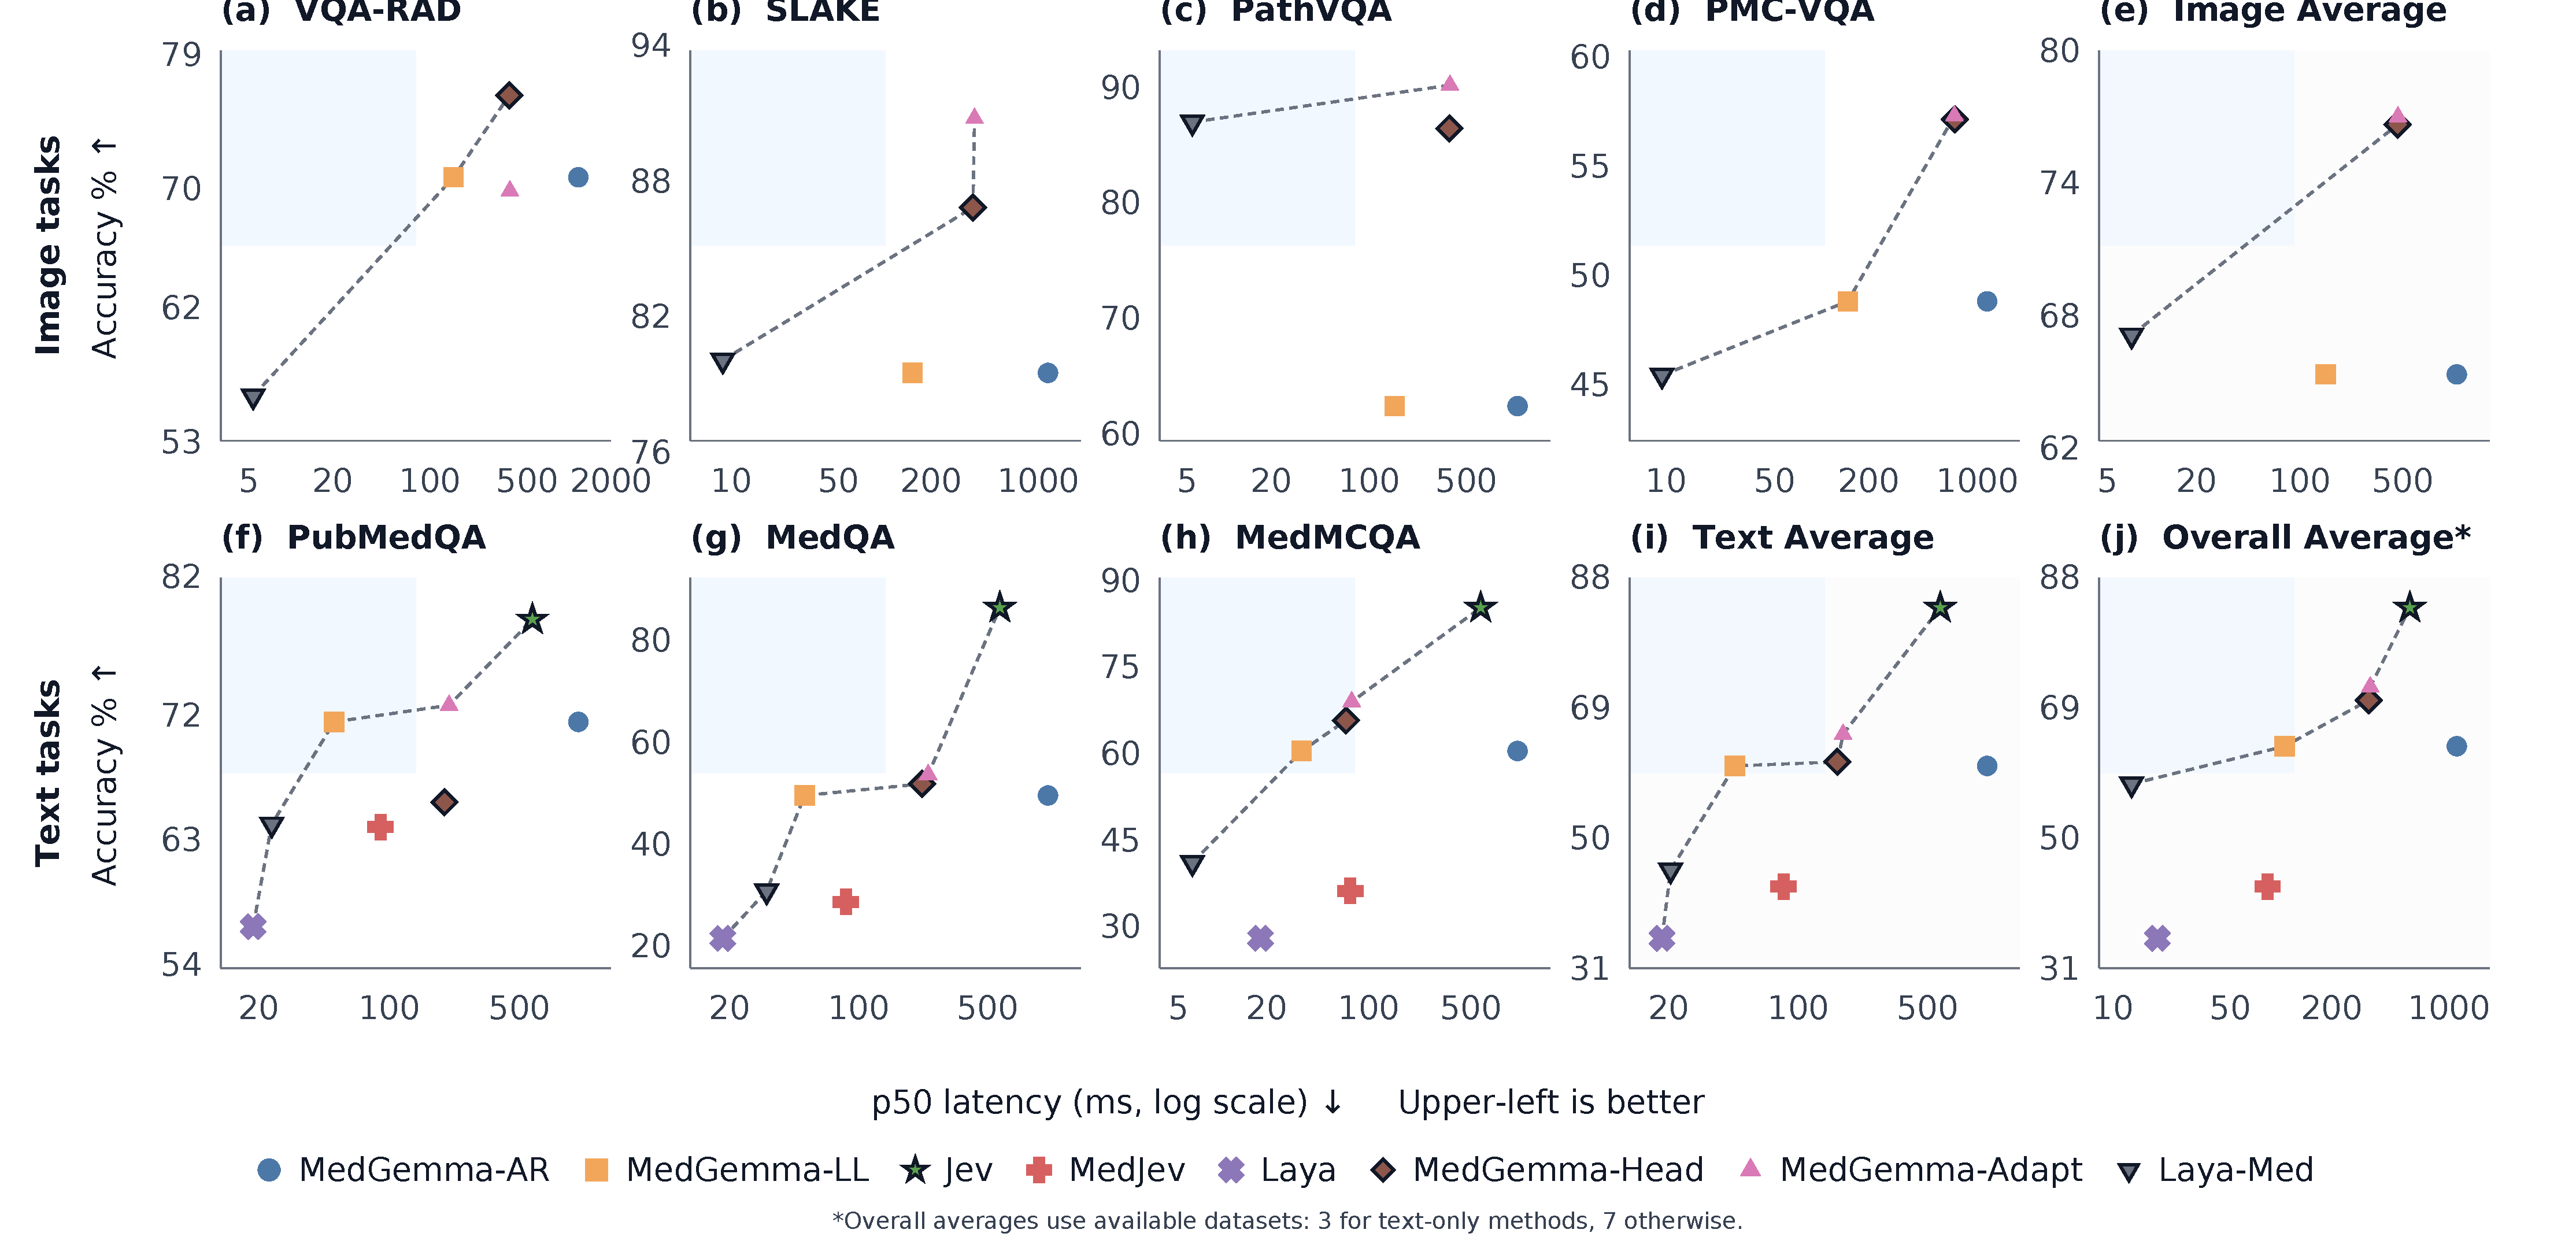
\includegraphics[width=\textwidth]{assets/figures/accuracy_latency_pareto.pdf}
\caption{Accuracy and median latency for AR-Gen and AR-LL. Native label scoring preserves observed choice accuracy while substantially reducing measured latency.}
\label{fig:accuracy_latency}
\end{figure*}

\subsection{What Is Gained by Removing Autoregressive Decoding?}
\label{sec:rq1}
\researchquestion[AR-LL preserves the observed choice while removing most of the measured decoding cost.]{Question 1}{What is gained by replacing answer generation with direct candidate scoring?}

\textbf{The decision is unchanged; the route to it is shorter.} Across the seven evaluated datasets, AR-Gen and AR-LL have the same accuracy in the reference landscape. Their macro accuracies are both 63.1\%, while the mean of per-dataset median latency falls from 1,114\,ms to 105\,ms. The points therefore move left, not up: in this MedGemma comparison, replacing answer-token generation changes the cost of obtaining the choice, not which choice is selected. The paired error analysis likewise finds identical AR-Gen and AR-LL outcomes. This is the cleanest within-backbone contrast in the study, but its timing remains an implementation measurement rather than a hardware-controlled claim about all AR and likelihood systems.

The broader implication is deliberately limited. A bounded output space can make sequential decoding unnecessary, but avoiding decoding alone does not repair errors or improve the confidence distribution: AR-Gen and AR-LL have identical paired probability vectors and error sets under this setup. Gains in decision quality require a change beyond the scoring route itself.

\subsection{When Does Learning the Decision Interface Help?}
\label{sec:rq2}
\researchquestion[AR-Head changes the decision boundary; AR-Adapt adds a smaller, nonuniform benefit.]{Question 2}{When do a learned scoring head and backbone adaptation improve bounded decisions?}

\textbf{A learned interface helps, but not on every task.} In the evaluated landscape, AR-Head raises macro accuracy from 63.1\% for AR-LL to 69.8\%; AR-Adapt reaches 71.8\%. The paired, example-weighted contrast is larger for AR-LL versus AR-Head (+9.5 percentage points, 95\% CI [8.5, 10.6]) than the macro difference: the pooled estimate gives more weight to larger benchmarks, where gains are strongest, particularly PathVQA and PMC-VQA. The gain is not universal: AR-Head is lower on PubMedQA, while improvements range from modest on MedQA and VQA-RAD to substantial on PathVQA. This pattern suggests that supervised candidate scoring is most useful when the pretrained generation interface is a poor fit to the benchmark's decision boundary, rather than providing a fixed bonus across tasks.

\textbf{Adaptation is a refinement, not a guarantee.} Relative to AR-Head, AR-Adapt adds about two macro accuracy points and a +2.5-point example-weighted paired effect (95\% CI [1.6, 3.5]). The direction varies by dataset: gains appear on PubMedQA, MedMCQA, SLAKE, and PathVQA, while VQA-RAD trends downward and MedQA and PMC-VQA show little separation. The useful conclusion is not that LoRA adaptation always helps, but that AR-Adapt can shift which examples are solved after a head has learned the bounded interface.

\begin{figure*}[t]
\centering

\begin{minipage}[t]{0.485\textwidth}
    \centering
    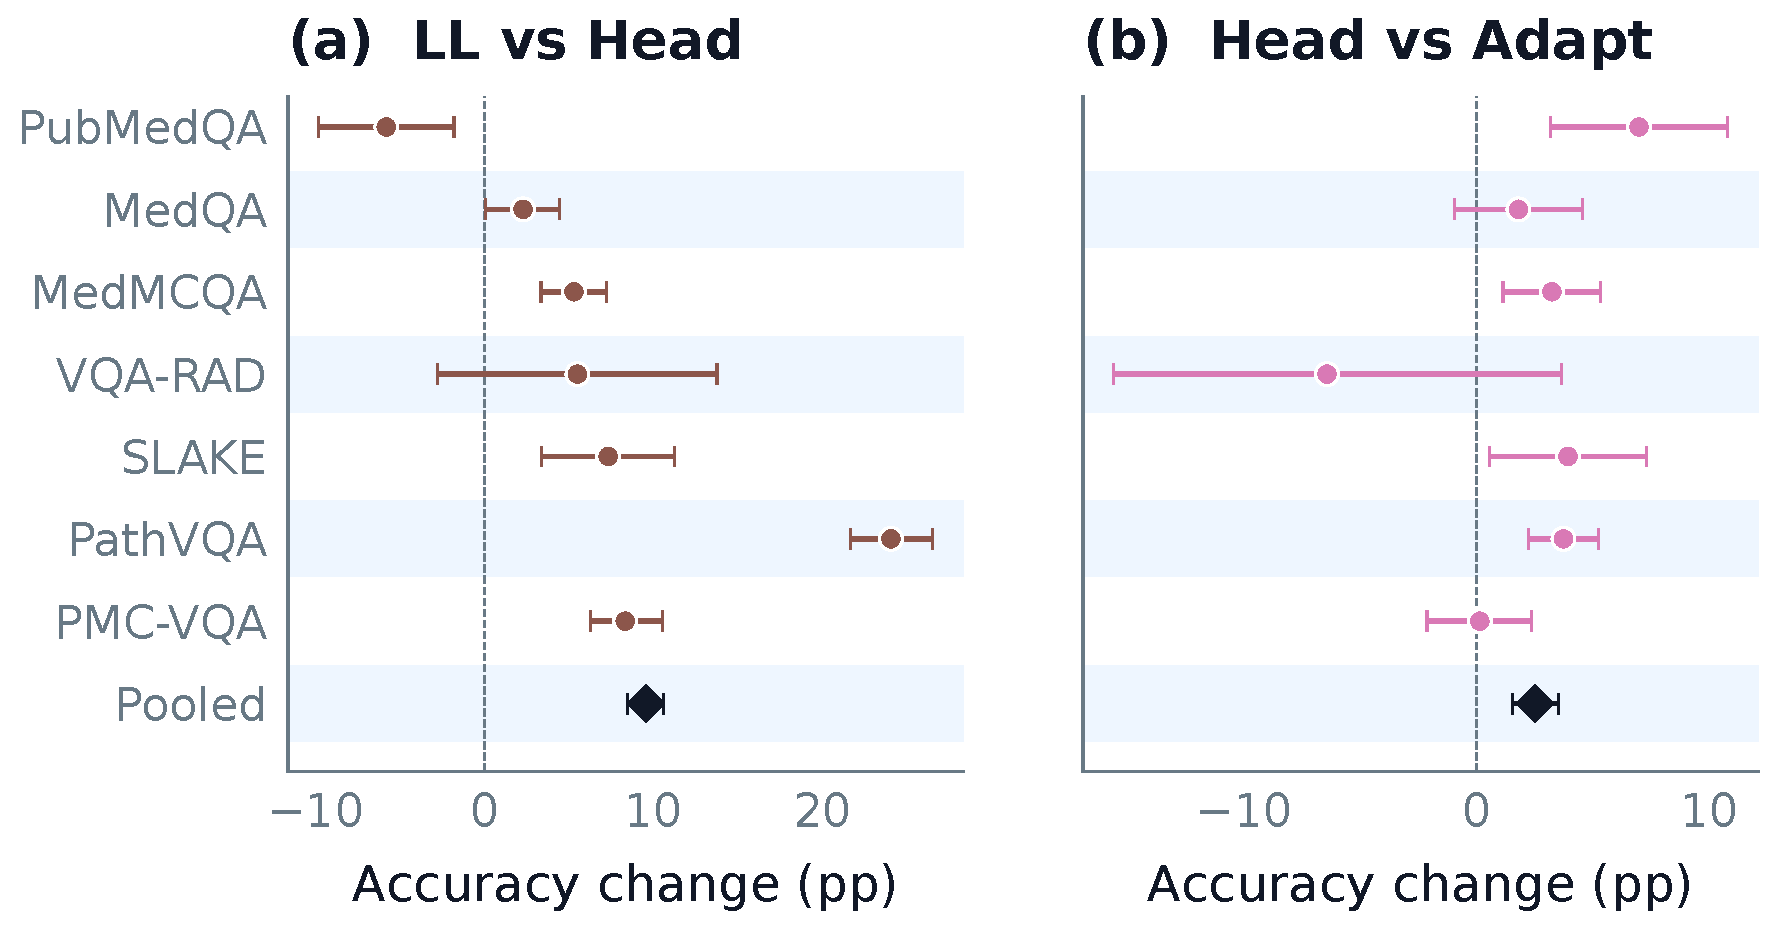
\includegraphics[
        width=\linewidth,
        trim=0 0 0 0,
        clip
    ]{assets/figures/paired_accuracy_effects.pdf}

    \captionof{figure}{
    \textbf{Paired accuracy effects.}
    Accuracy differences on matched examples; diamonds denote
    pooled effects and whiskers show 95\% paired bootstrap intervals.
    }
    \label{fig:paired_effects}
\end{minipage}
\hfill
\begin{minipage}[t]{0.485\textwidth}
    \centering
    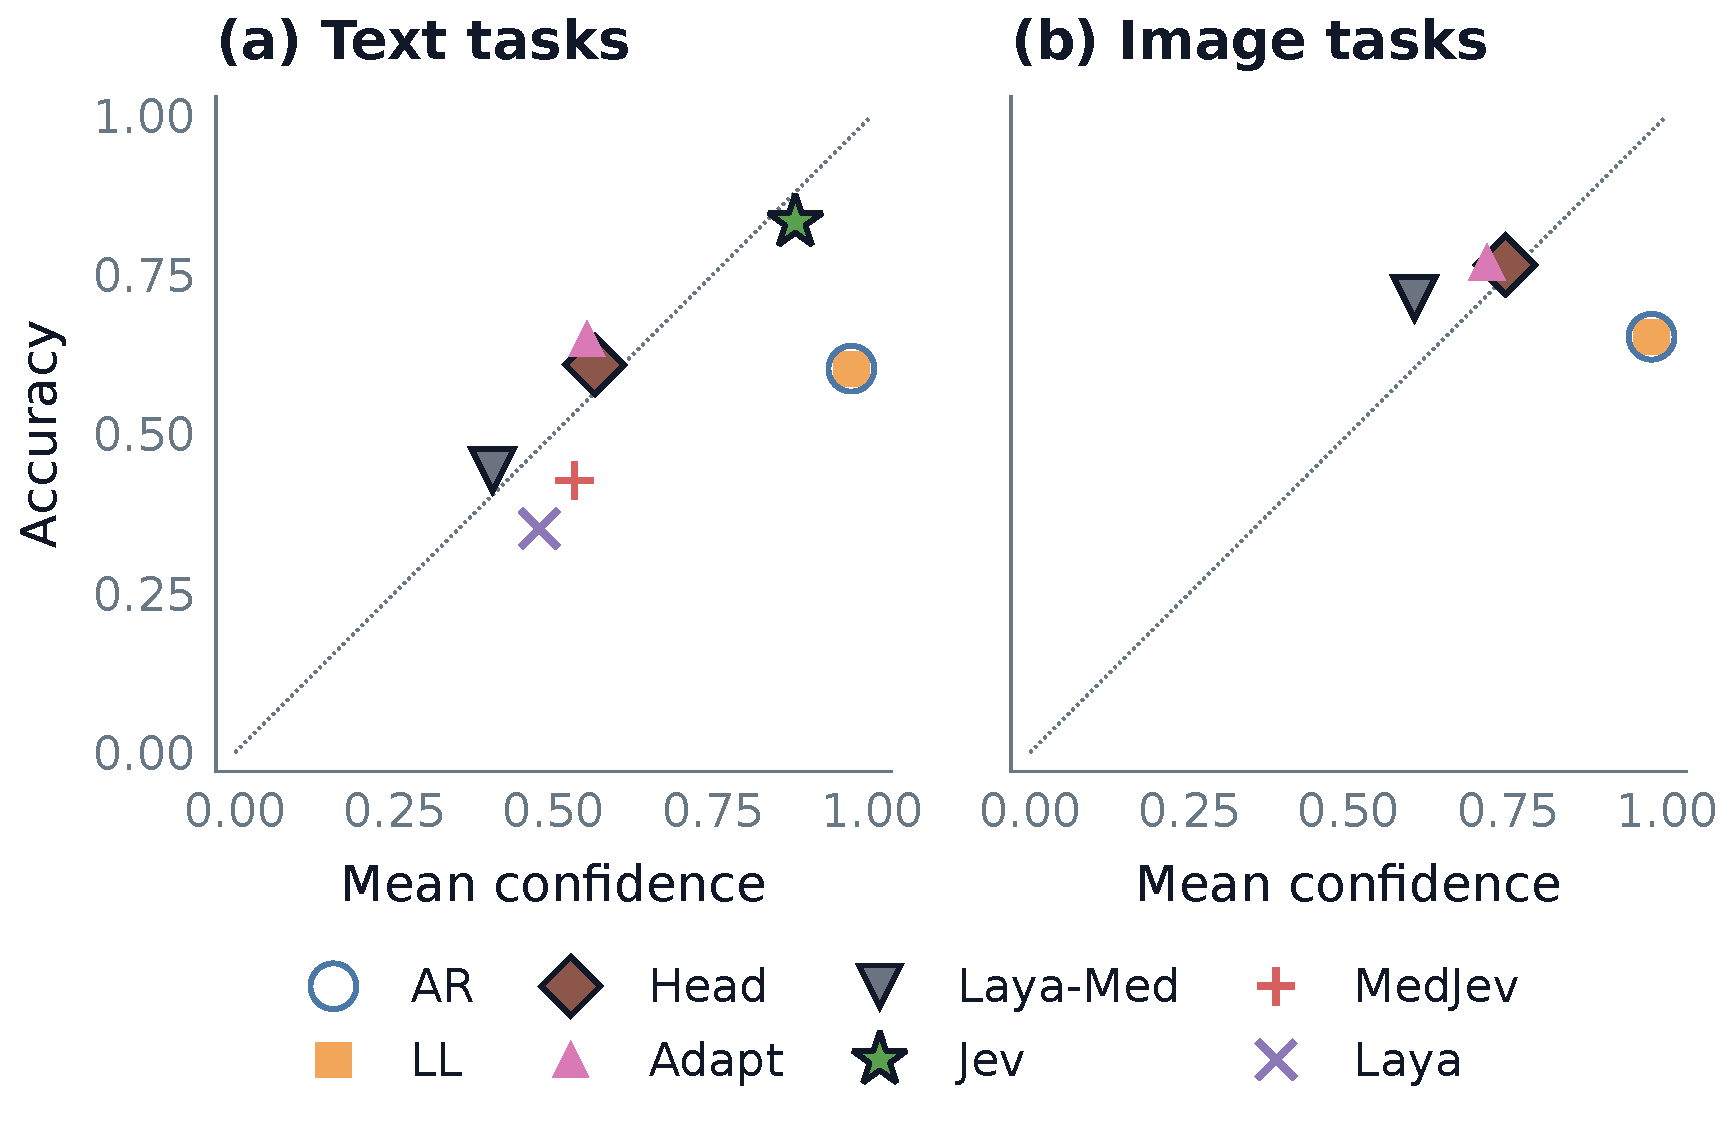
\includegraphics[
        width=0.81\linewidth,
        trim=0 0 0 0,
        clip
    ]{assets/figures/figure4_mean_confidence_accuracy.pdf}

    \captionof{figure}{
    \textbf{Confidence--accuracy alignment.}
    Mean confidence versus accuracy by modality; the diagonal denotes perfect mean alignment.
    }
    \label{fig:mean_confidence}
\end{minipage}

\end{figure*}

\textbf{Accuracy and probability quality can move in opposite directions.} The probability landscape shows that AR-Head improves accuracy, ECE, NLL, and Brier score relative to AR-LL. AR-Adapt then raises accuracy further, while its macro ECE and NLL are worse than those of AR-Head. A more accurate argmax therefore need not come with a better probability distribution. This distinction matters because routing and conformal prediction use the distribution, not accuracy alone, to decide which examples to retain.

\begin{figure*}[t]
\centering
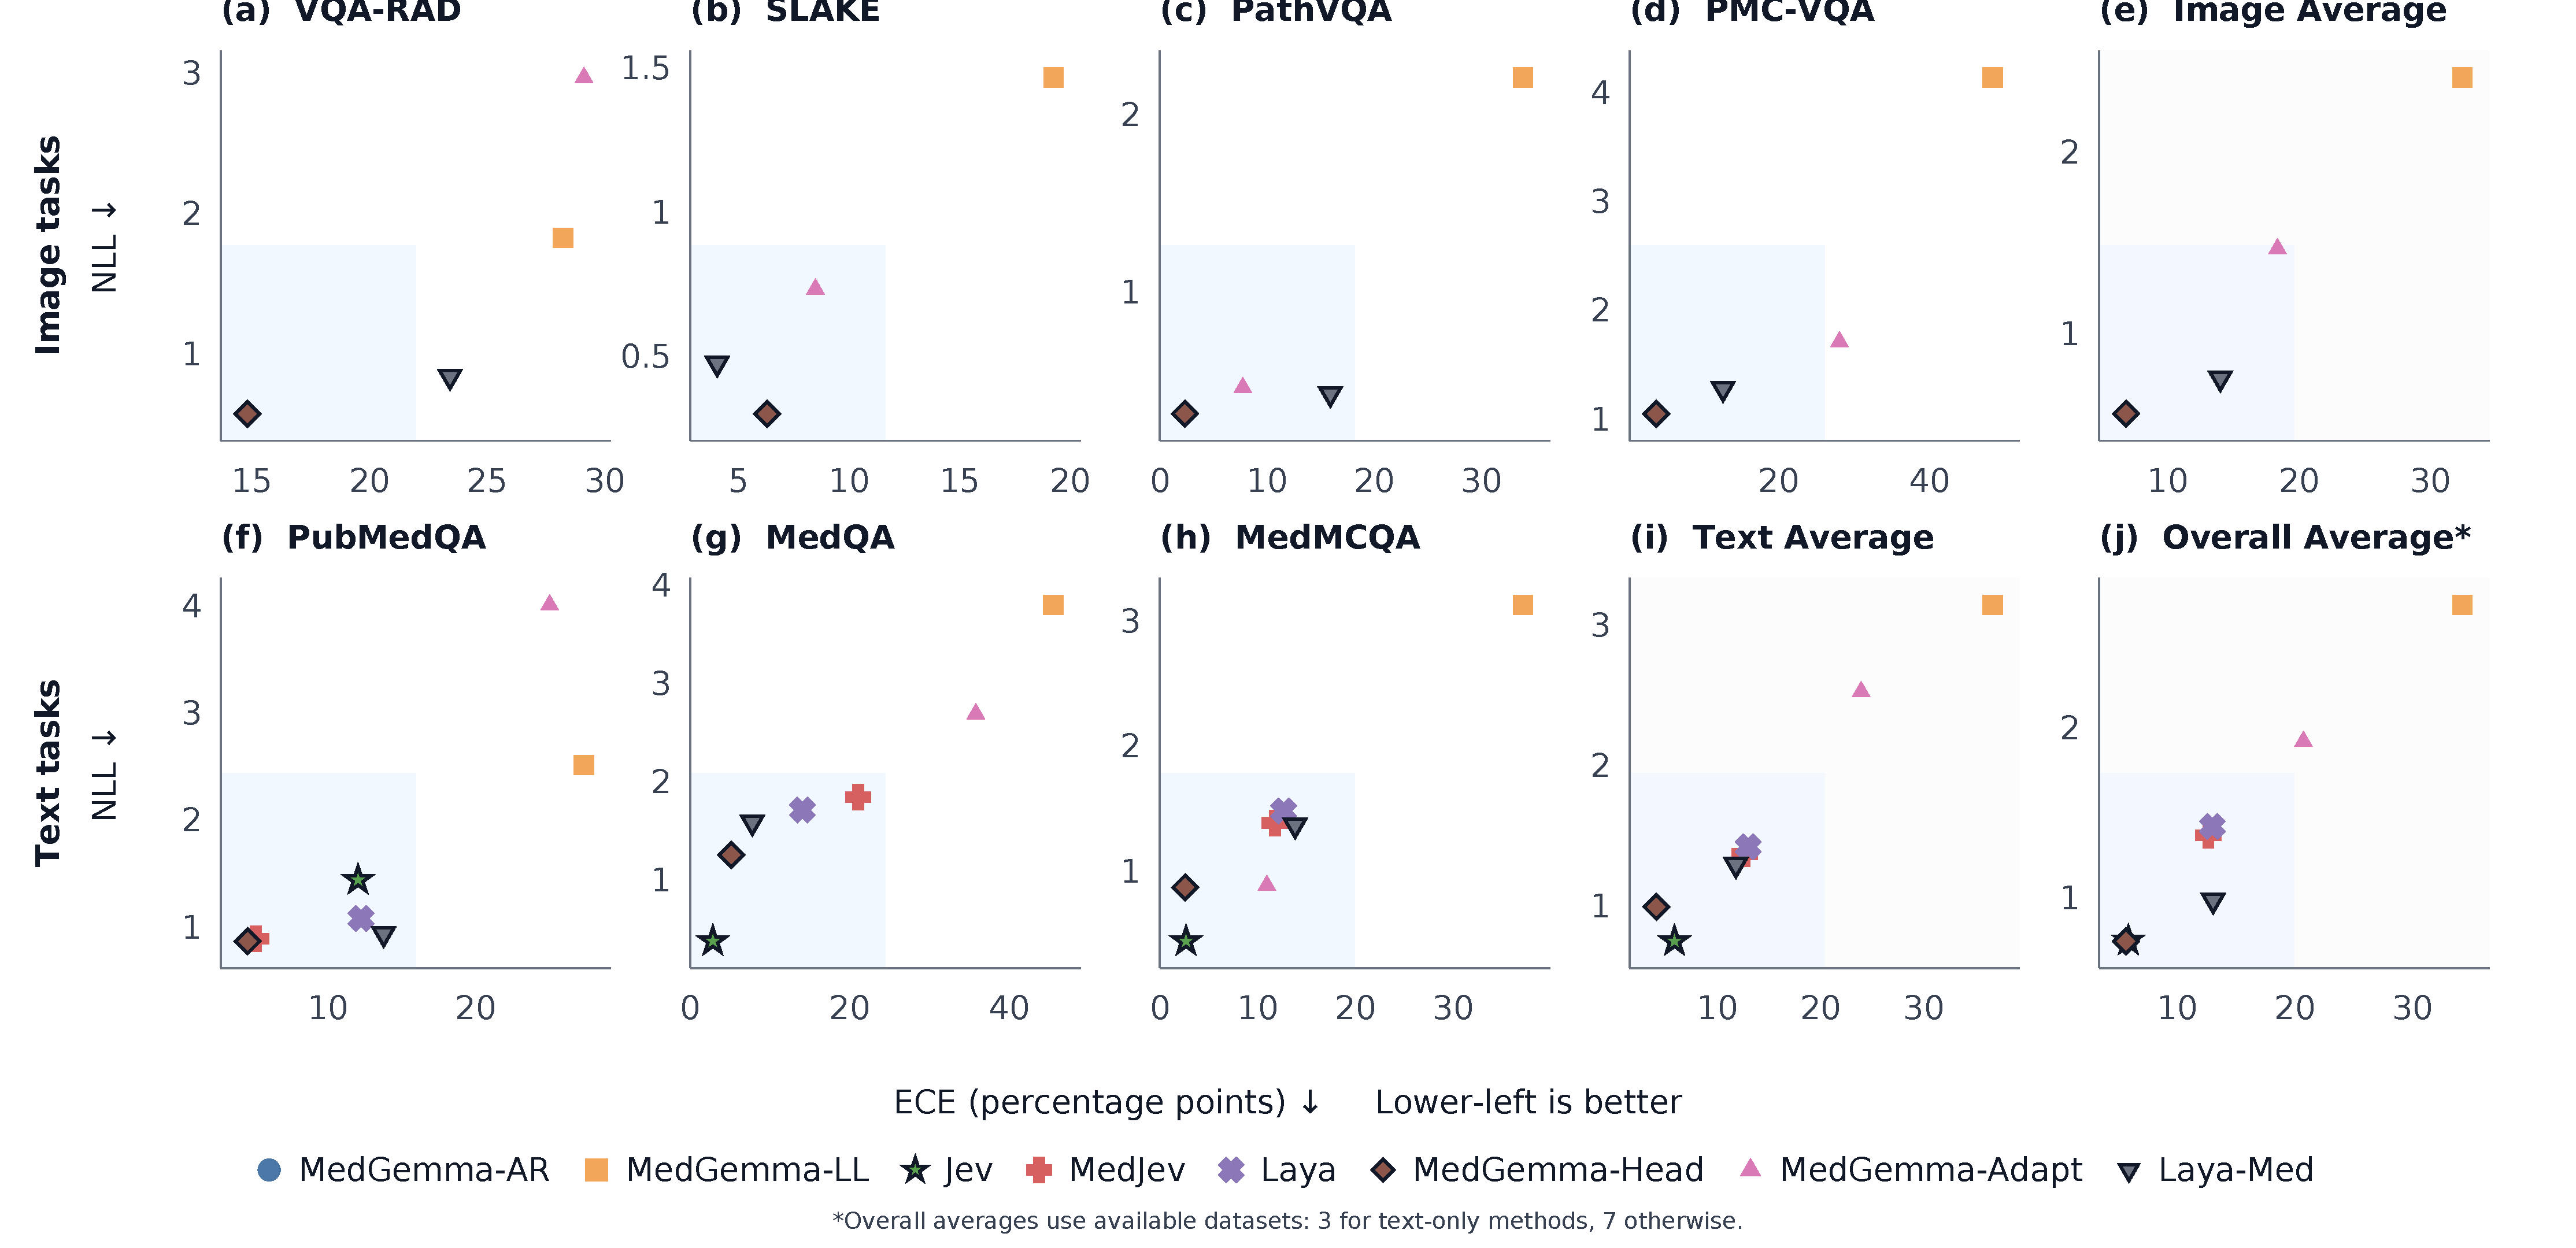
\includegraphics[width=\textwidth]{assets/figures/ece_nll_pareto.pdf}
\caption{Calibration--likelihood landscape for the configured test evaluations. Lower ECE and NLL are better.}
\label{fig:ece_nll_pareto}
\end{figure*}

\textbf{Confidence is a ranking signal, not just a mean.} In the confidence--accuracy comparison, AR-Gen and AR-LL have mean confidence well above accuracy on both text and image tasks. AR-Head and AR-Adapt are closer to the diagonal, while NAR-Med (Laya-Med) is underconfident on average. These modality-level means summarize different confidence distributions and should not be read as calibration guarantees. Jev, MedJev, and NAR (Laya) provide text-only context, but their implementations make them unsuitable as controlled contrasts. The selective analyses below test whether confidence separates correct from incorrect predictions.

\subsection{How Do AR- and NAR-Based Decision Systems Compare?}
\label{sec:rq3}
\researchquestion[NAR-Med is fast, but its accuracy and visual reliance depend strongly on the dataset.]{Question 3}{What trade-offs appear across representations and modalities?}

\textbf{Fast decisions do not imply uniform competence.} NAR-Med (Laya-Med) has the lowest measured latency in the landscape, but its macro accuracy (57.6\%) trails AR-Head and AR-Adapt. Its behavior is sharply task-dependent: it is competitive on SLAKE and PathVQA, but substantially weaker on MedQA, MedMCQA, and PMC-VQA. The gap is not captured by a simple text-versus-image split: even among image benchmarks, VQA-RAD and PMC-VQA remain difficult while SLAKE and PathVQA are much stronger. This points to benchmark-specific candidate structure and visual-question demands as more informative than modality alone. Because backbone, pretraining, fusion, and implementation differ, these measurements characterize the systems evaluated rather than isolating an architecture-only effect.

\textbf{Similar averages conceal different errors.} AR-Gen and AR-LL make identical decisions, but the learned methods redistribute errors across examples. AR-Head and AR-Adapt disagree in correctness on 20.6\% of cases; AR-Adapt and NAR-Med (Laya-Med) disagree on 31.5\%. The latter pair also fails together on 20.7\% of cases. This is evidence of complementary outcomes, not yet an ensemble: a useful selector would need an independently available signal that identifies which model is right on each example.

\begin{figure*}[t]
\centering

% ============================================================
% LEFT FIGURE
% ============================================================
\begin{minipage}[t]{0.485\textwidth}
    \centering

    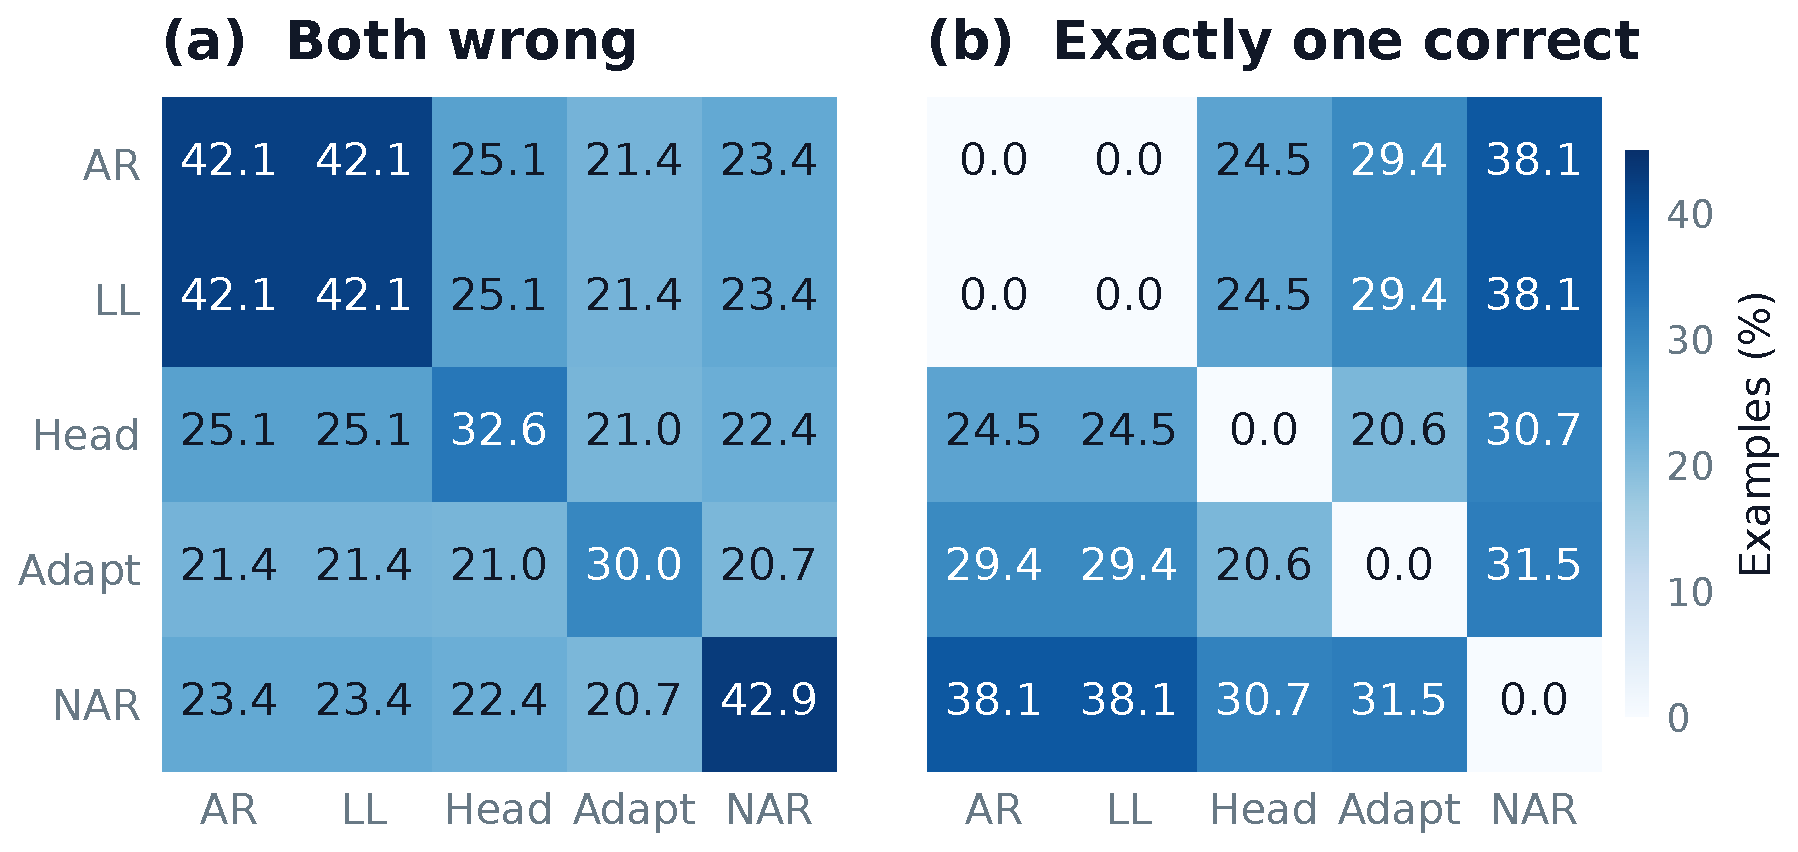
\includegraphics[
        width=\linewidth,
        trim=0 0 0 0,
        clip
    ]{assets/figures/figure3_four_formulation_error_overlap.pdf}

    \captionof{figure}{
    \textbf{Paired error overlap.}
    Both-method errors and cases where exactly one method is correct
    on matched test examples.
    }
    \label{fig:error_overlap}
\end{minipage}
\hfill
% ============================================================
% RIGHT FIGURE
% ============================================================
\begin{minipage}[t]{0.485\textwidth}
    \centering

    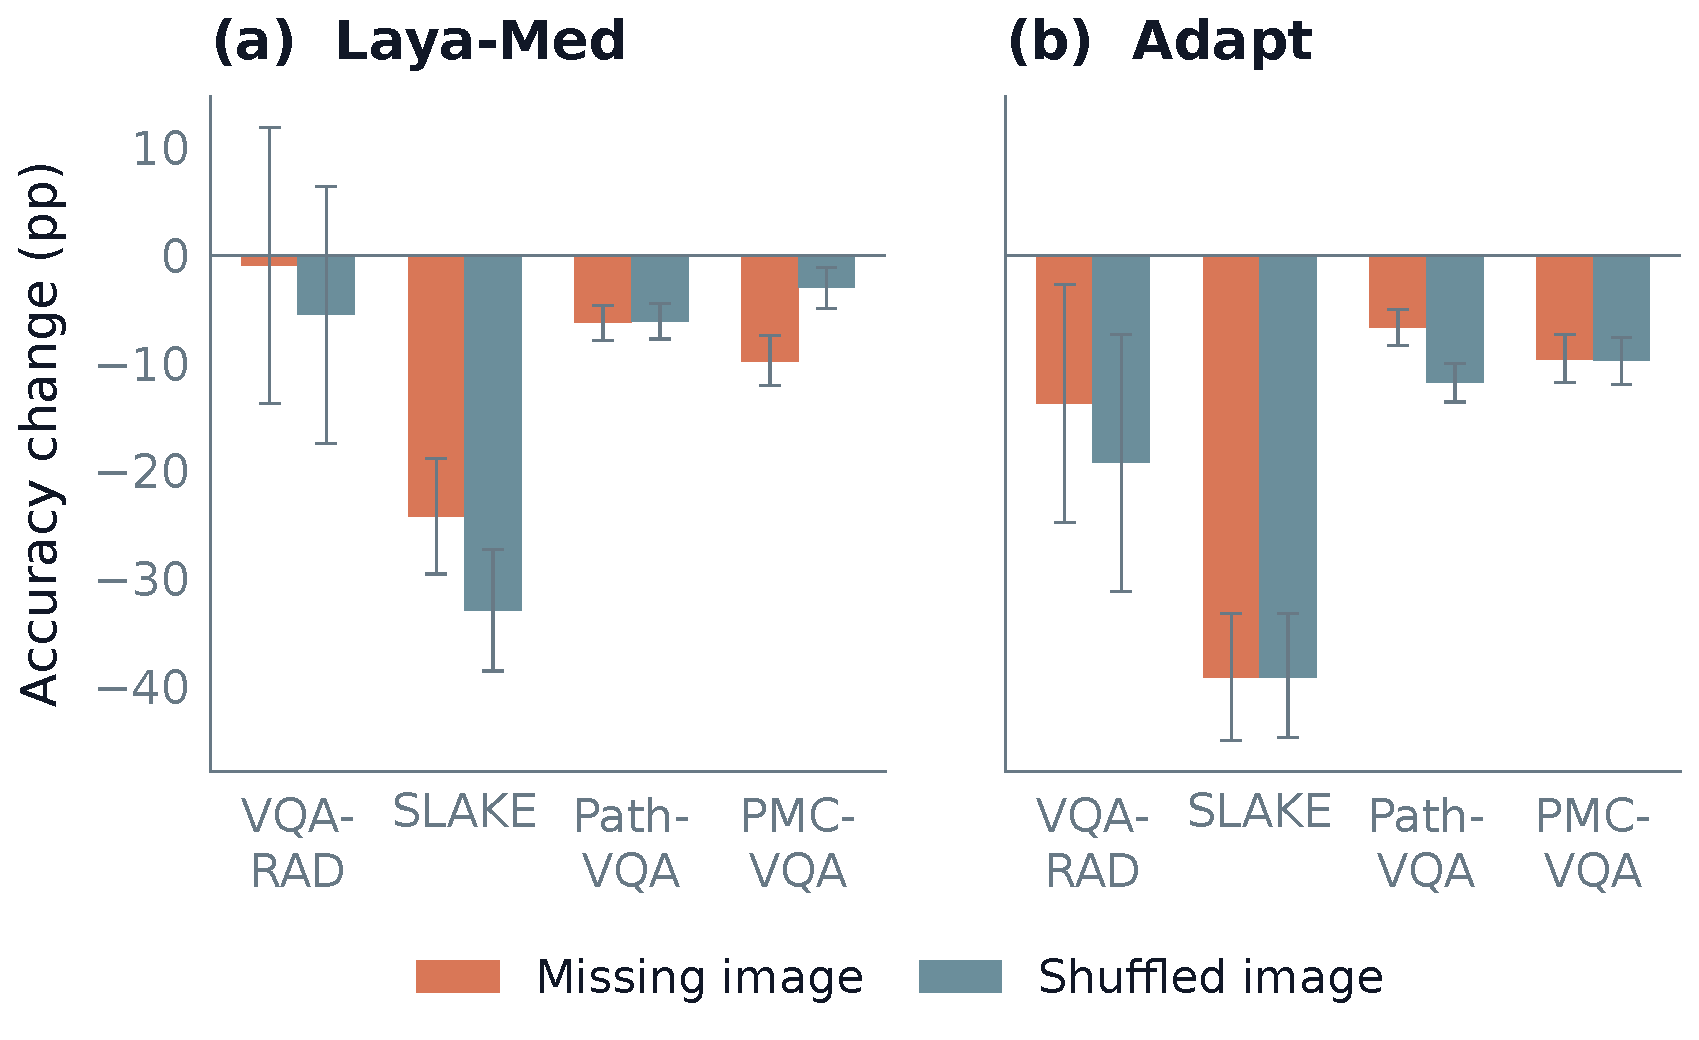
\includegraphics[
        width=0.77\linewidth,
        trim=0 0 0 0,
        clip
    ]{assets/figures/visual_dependence_ablation.pdf}

    \captionof{figure}{
    \textbf{Visual dependence.}
    Accuracy changes after removing or shuffling images relative
    to the correct-image condition; whiskers show 95\% paired
    bootstrap intervals.
    }
    \label{fig:visual_dependence}
\end{minipage}

\end{figure*}

\textbf{Benchmark accuracy is not proof of image use.} The ablations make this distinction concrete. NAR-Med is highly sensitive to removing or shuffling SLAKE images, but its PathVQA accuracy falls by only about six points under either perturbation; its VQA-RAD changes are smaller and uncertain. AR-Adapt shows substantial sensitivity on SLAKE and PMC-VQA, with more moderate but consistent drops on PathVQA and VQA-RAD. The contrast indicates that visual evidence contributes differently across datasets and models. It also cautions against interpreting image-task accuracy as evidence that a model relied on the image: perturbation effects, not task labels alone, reveal that dependence.

\begin{table*}[t]
\centering\scriptsize
\setlength{\tabcolsep}{3.2pt}
\renewcommand{\arraystretch}{1.20}
\begin{tabular*}{\textwidth}{@{\extracolsep{\fill}}lrrrrrrrr@{}}
\toprule
Formulation / policy & PubMedQA & MedQA & MedMCQA & VQA-RAD & SLAKE & PathVQA & PMC-VQA & Avg. \\
\midrule
\textbf{AR-LL} & 71.2 & 49.4 & 60.0 & 70.6 & 79.4 & 62.4 & 48.9 & 63.1 \\
\quad + Routing & 72.5$^{2.4}$ & 50.8$^{6.9}$ & 60.9$^{3.0}$ & 71.3$^{0.9}$ & 80.1$^{2.5}$ & 63.1$^{4.2}$ & 49.6$^{3.1}$ & 64.0$^{3.3}$ \\
\quad + Conformal & 75.5$^{11.2}$ & 56.4$^{35.3}$ & 65.8$^{22.0}$ & 77.4$^{14.7}$ & 82.4$^{13.5}$ & 67.1$^{29.6}$ & 53.8$^{24.8}$ & 68.3$^{21.6}$ \\
\addlinespace[3pt]
\textbf{MedJev} & 63.8 & 28.3 & 35.9 & -- & -- & -- & -- & 42.7 \\
\quad + Routing & \textbf{76.5}$^{66.0}$ & 33.3$^{86.8}$ & 56.9$^{92.8}$ & -- & -- & -- & -- & 55.6$^{81.9}$ \\
\quad + Conformal & 68.6$^{34.4}$ & 32.5$^{60.4}$ & 44.0$^{68.2}$ & -- & -- & -- & -- & 48.4$^{54.3}$ \\
\addlinespace[3pt]
\textbf{NAR (Laya)} & 56.6 & 21.1 & 27.6 & -- & -- & -- & -- & 35.1 \\
\quad + Routing & 65.2$^{48.8}$ & 37.5$^{98.1}$ & 21.6$^{97.5}$ & -- & -- & -- & -- & 41.4$^{81.5}$ \\
\quad + Conformal & 61.3$^{22.0}$ & 23.1$^{80.2}$ & 30.1$^{76.0}$ & -- & -- & -- & -- & 38.2$^{59.4}$ \\
\addlinespace[3pt]
\textbf{AR-Head} & 65.6 & 51.5 & 65.5 & 76.1 & 86.8 & 86.3 & 57.1 & 69.8 \\
\quad + Routing & 75.9$^{51.0}$ & \textbf{77.0}$^{75.0}$ & \textbf{87.4}$^{56.7}$ & \textbf{78.1}$^{41.3}$ & 89.3$^{7.9}$ & 91.4$^{15.4}$ & \textbf{77.7}$^{71.4}$ & \textbf{82.4}$^{45.5}$ \\
\quad + Conformal & 68.1$^{13.4}$ & 55.0$^{21.5}$ & 69.1$^{12.7}$ & 77.2$^{7.3}$ & 87.2$^{1.1}$ & 87.6$^{3.0}$ & 61.5$^{16.0}$ & 72.3$^{10.7}$ \\
\addlinespace[3pt]
\textbf{AR-Adapt} & 72.6 & 53.3 & 68.7 & 69.7 & 90.7 & 90.0 & 57.2 & 71.8 \\
\quad + Routing & 73.0$^{3.0}$ & 57.1$^{16.0}$ & 81.7$^{32.9}$ & 70.4$^{0.9}$ & \textbf{91.6}$^{2.5}$ & 91.0$^{3.2}$ & 61.5$^{21.2}$ & 75.2$^{11.4}$ \\
\quad + Conformal & 72.9$^{0.4}$ & 54.1$^{3.9}$ & 72.0$^{9.4}$ & 69.7$^{0.0}$ & 91.4$^{1.4}$ & 90.4$^{1.0}$ & 58.2$^{5.9}$ & 72.7$^{3.1}$ \\
\addlinespace[3pt]
\textbf{NAR-Med (Laya-Med)} & 64.0 & 30.4 & 40.8 & 56.0 & 80.0 & 86.8 & 45.4 & 57.6 \\
\quad + Routing & 69.1$^{21.0}$ & --$^{100.0}$ & --$^{100.0}$ & 60.2$^{23.9}$ & 84.7$^{24.5}$ & \textbf{95.8}$^{45.1}$ & --$^{100.0}$ & 77.5$^{59.2}$ \\
\quad + Conformal & 64.3$^{0.4}$ & 31.7$^{70.7}$ & 54.6$^{73.0}$ & 56.7$^{4.6}$ & 80.4$^{0.8}$ & 87.1$^{1.0}$ & 49.4$^{28.3}$ & 60.6$^{25.5}$ \\
\addlinespace[3pt]
\bottomrule
\end{tabular*}
\caption{Reference TTA evaluation: accuracy (\%) with routing at $\tau=0.7$ and conformal singleton selection at $\alpha=0.3$. Superscripts give abstention percentages. Bold marks the highest accuracy in each column, including ties. Accuracy averages exclude tasks with no accepted predictions; abstention averages include them. Dashes denote unsupported tasks or no accepted predictions.}
\label{tab:tta_accuracy_abstention}
\end{table*}

\begin{figure*}[t]
\centering
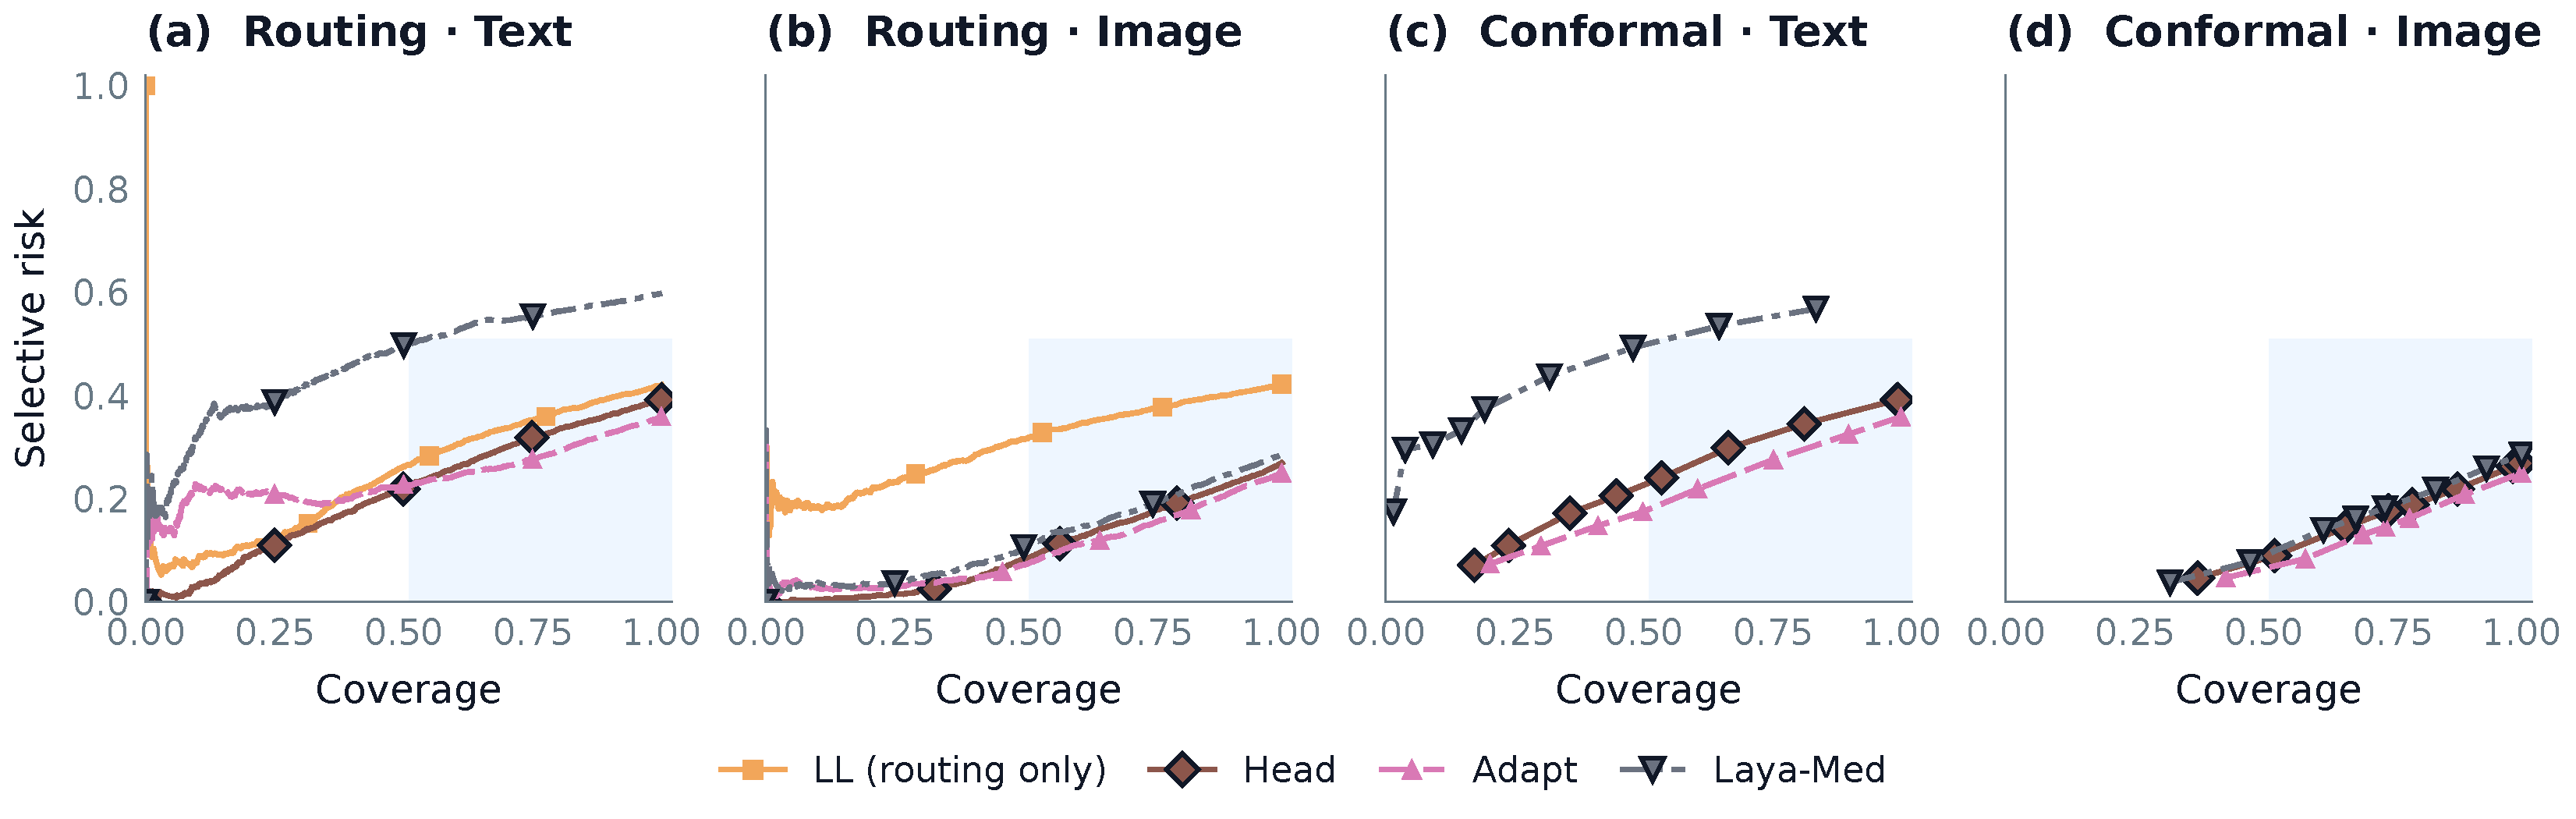
\includegraphics[width=\textwidth]{assets/figures/posthoc_risk_coverage_policies.pdf}
\caption{Selective risk--coverage by policy and modality. Routing sweeps confidence thresholds; conformal curves vary $\alpha$ and are shown for methods with independent calibration predictions. AR-LL contributes routing only; curves correspond to AR-LL, AR-Head, AR-Adapt, and NAR-Med.}
\label{fig:policy_comparison}
\end{figure*}

\subsection{Can Post-hoc Decision Policies Improve a Fixed Decision Model?}
\label{sec:rq4}
\researchquestion[Selective policies can improve accepted accuracy, but the gain is purchased with method- and task-dependent abstention.]{Question 4}{How can fixed decision distributions support more selective predictions?}

\textbf{Accepted accuracy has a coverage price.} Table~\ref{tab:tta_accuracy_abstention} reports reference operating points. Routing raises accepted accuracy most sharply for AR-Head and NAR-Med, but average abstention is also high; NAR-Med routing abstains on nearly three fifths of decisions on average and defers every MedQA, MedMCQA, and PMC-VQA decision in this table. Its higher accepted accuracy therefore describes a more selective subset, not an improvement to full-coverage prediction. AR-Adapt changes less at these operating points because routing rejects fewer decisions. Conformal singleton selection exhibits the same exchange: retained fractions and accepted accuracy vary by method and benchmark. The table's accepted-accuracy averages omit datasets with no accepted predictions, while its abstention averages retain them; both columns are needed to interpret the result.

\textbf{Confidence ordering differs across methods and modalities.} The risk--coverage figure shows how selective risk changes as progressively less-confident decisions are deferred. Risk is the error fraction among accepted decisions, and coverage is the accepted fraction of the corresponding modality evaluation. Routing traces AR-LL, AR-Head, AR-Adapt, and NAR-Med. Per-dataset conformal traces are available for AR-Head, AR-Adapt, and NAR-Med because AR-LL has no independent calibration export. The curve shape, rather than a single operating point, reveals whether confidence concentrates errors among low-confidence predictions.

\textbf{Task-level selectivity and label coverage.} The NAR-Med risk--coverage curves show why modality averages can mislead: confidence ranking is more useful on some tasks than others, and low coverage does not guarantee low risk on every benchmark. These curves characterize which decisions are retained; they do not change full-evaluation accuracy.

\begin{figure*}[t]
\centering

% ============================================================
% LEFT FIGURE
% ============================================================
\begin{minipage}[t]{0.485\textwidth}
    \centering

    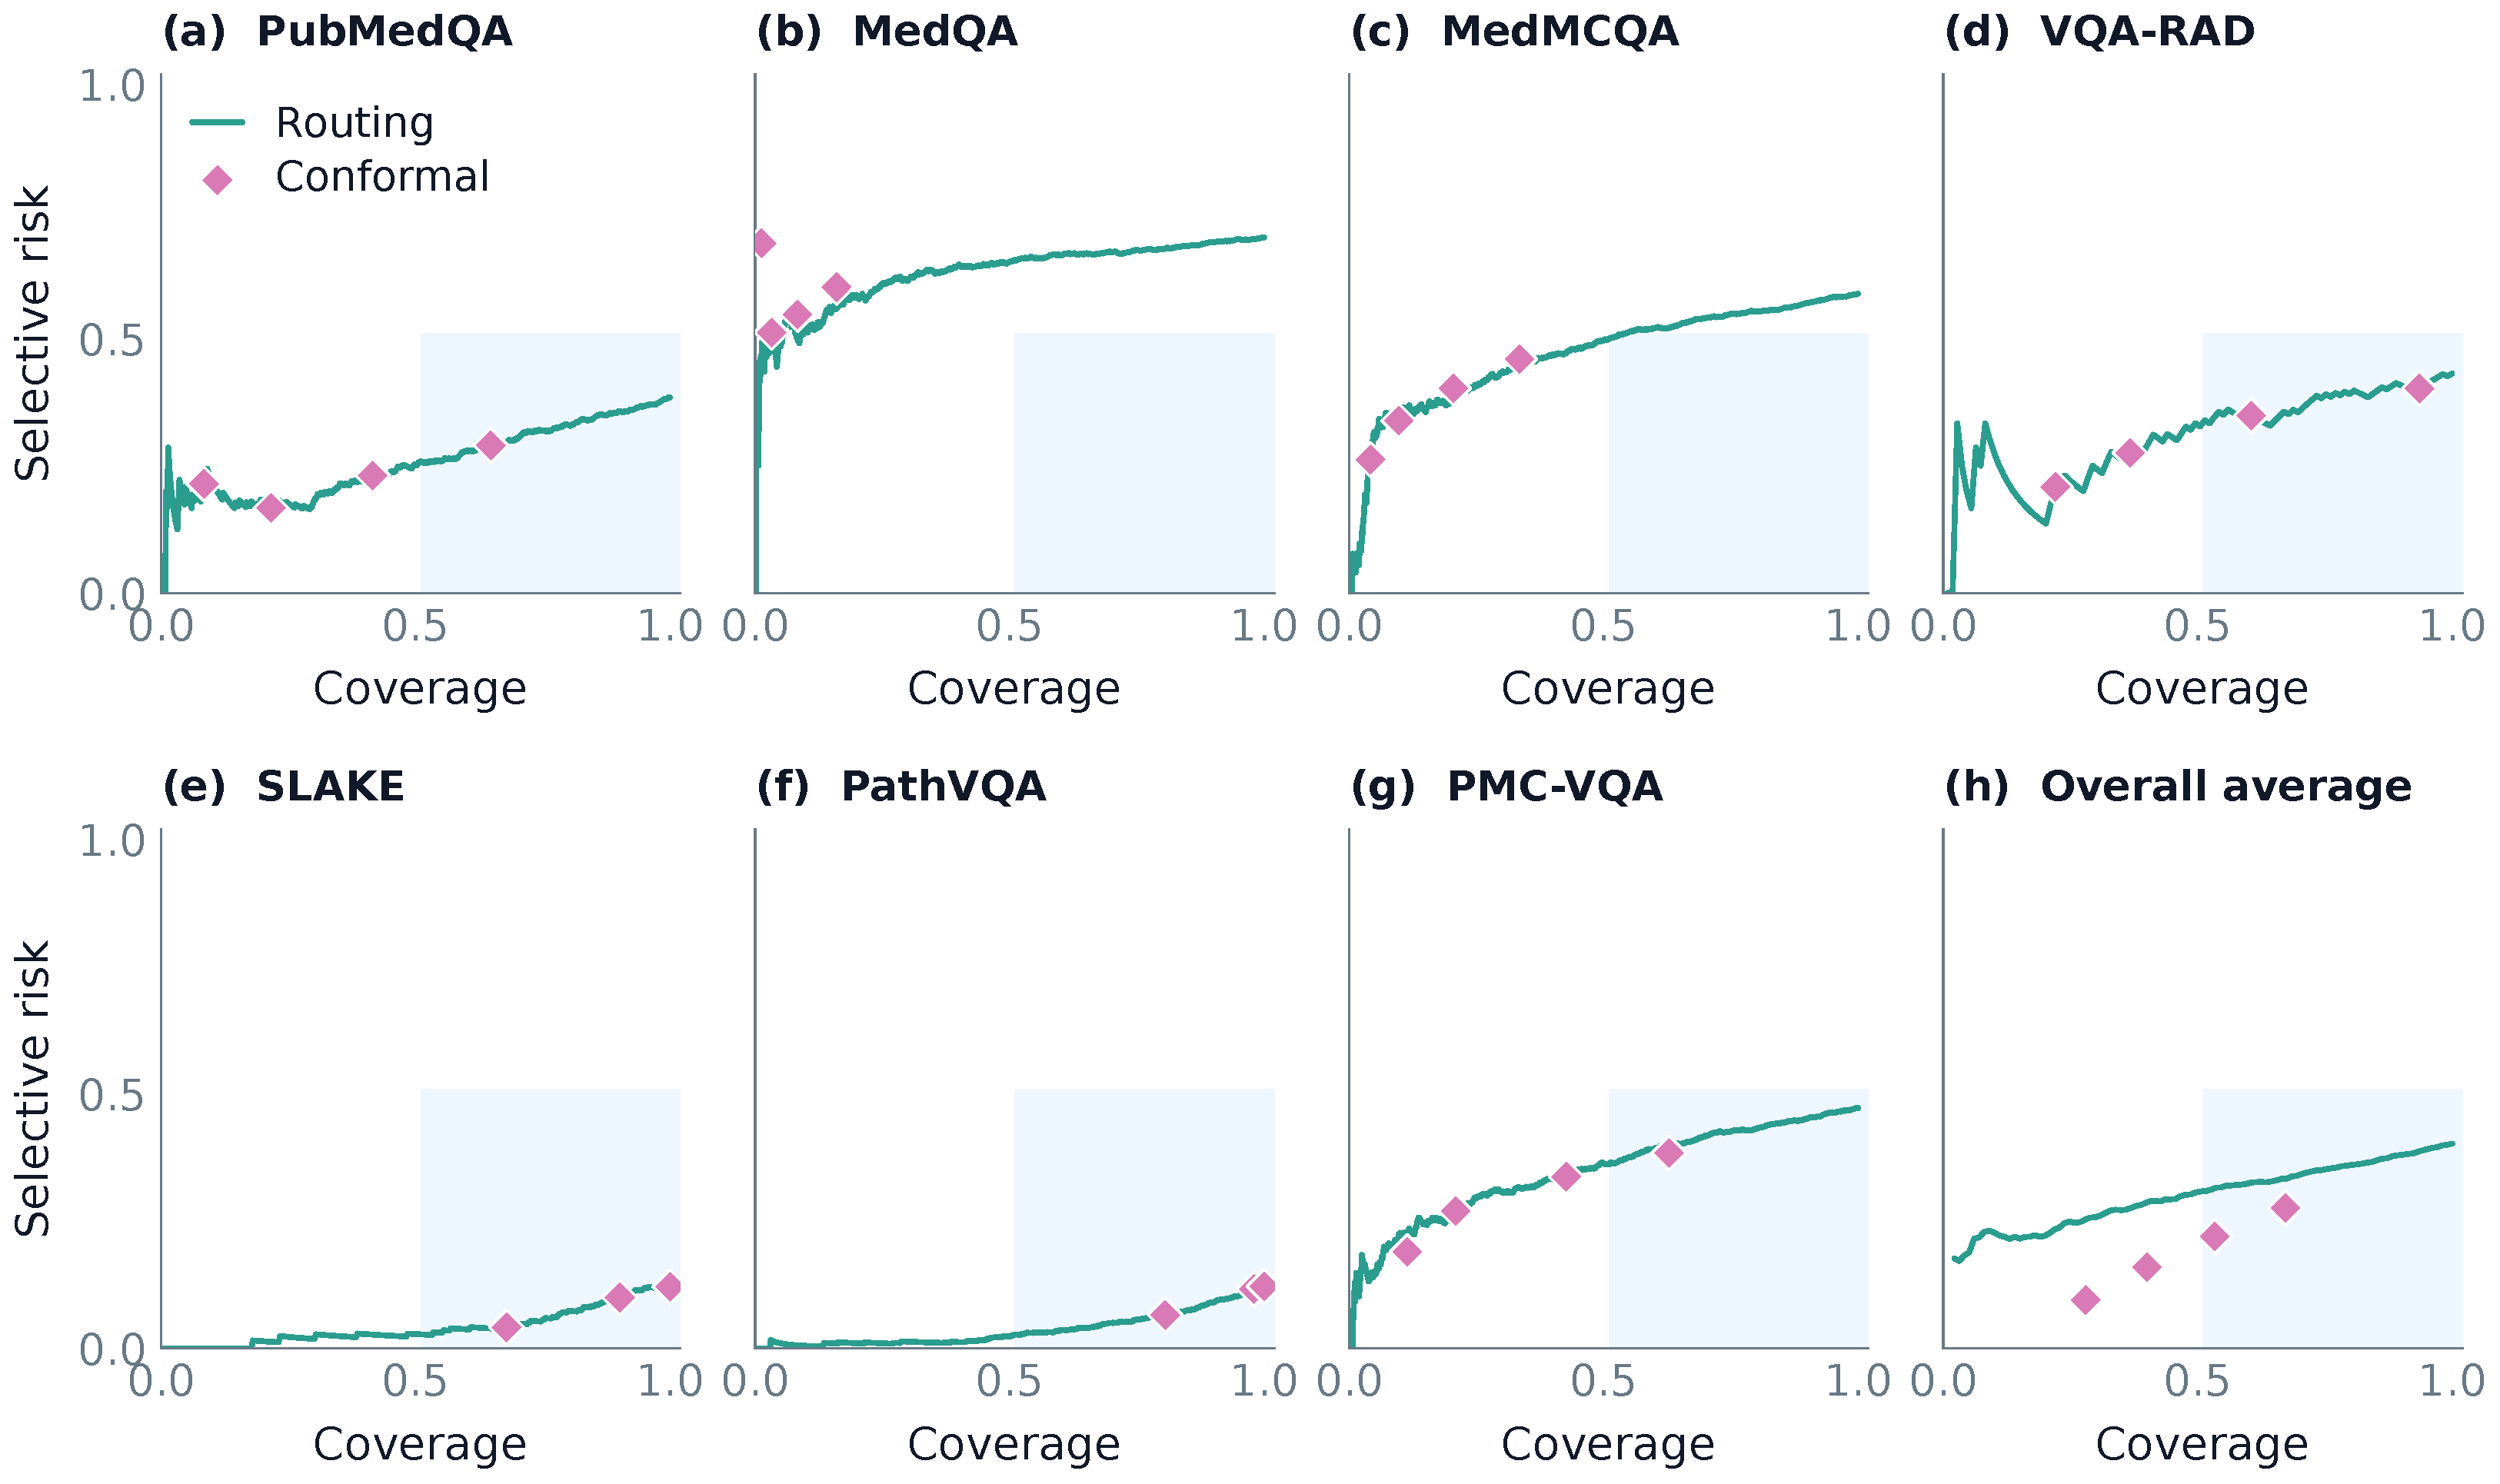
\includegraphics[
        width=\linewidth,
        trim=0 0 0 0,
        clip
    ]{assets/figures/posthoc_risk_coverage.pdf}

    \captionof{figure}{
    \textbf{Selective risk--coverage.}
    NAR-Med selective risk by dataset; lines show confidence-ranked
    decisions and diamonds denote conformal singleton operating points.
    }
    \label{fig:posthoc_risk}
\end{minipage}
\hfill
% ============================================================
% RIGHT FIGURE
% ============================================================
\begin{minipage}[t]{0.485\textwidth}
    \centering

    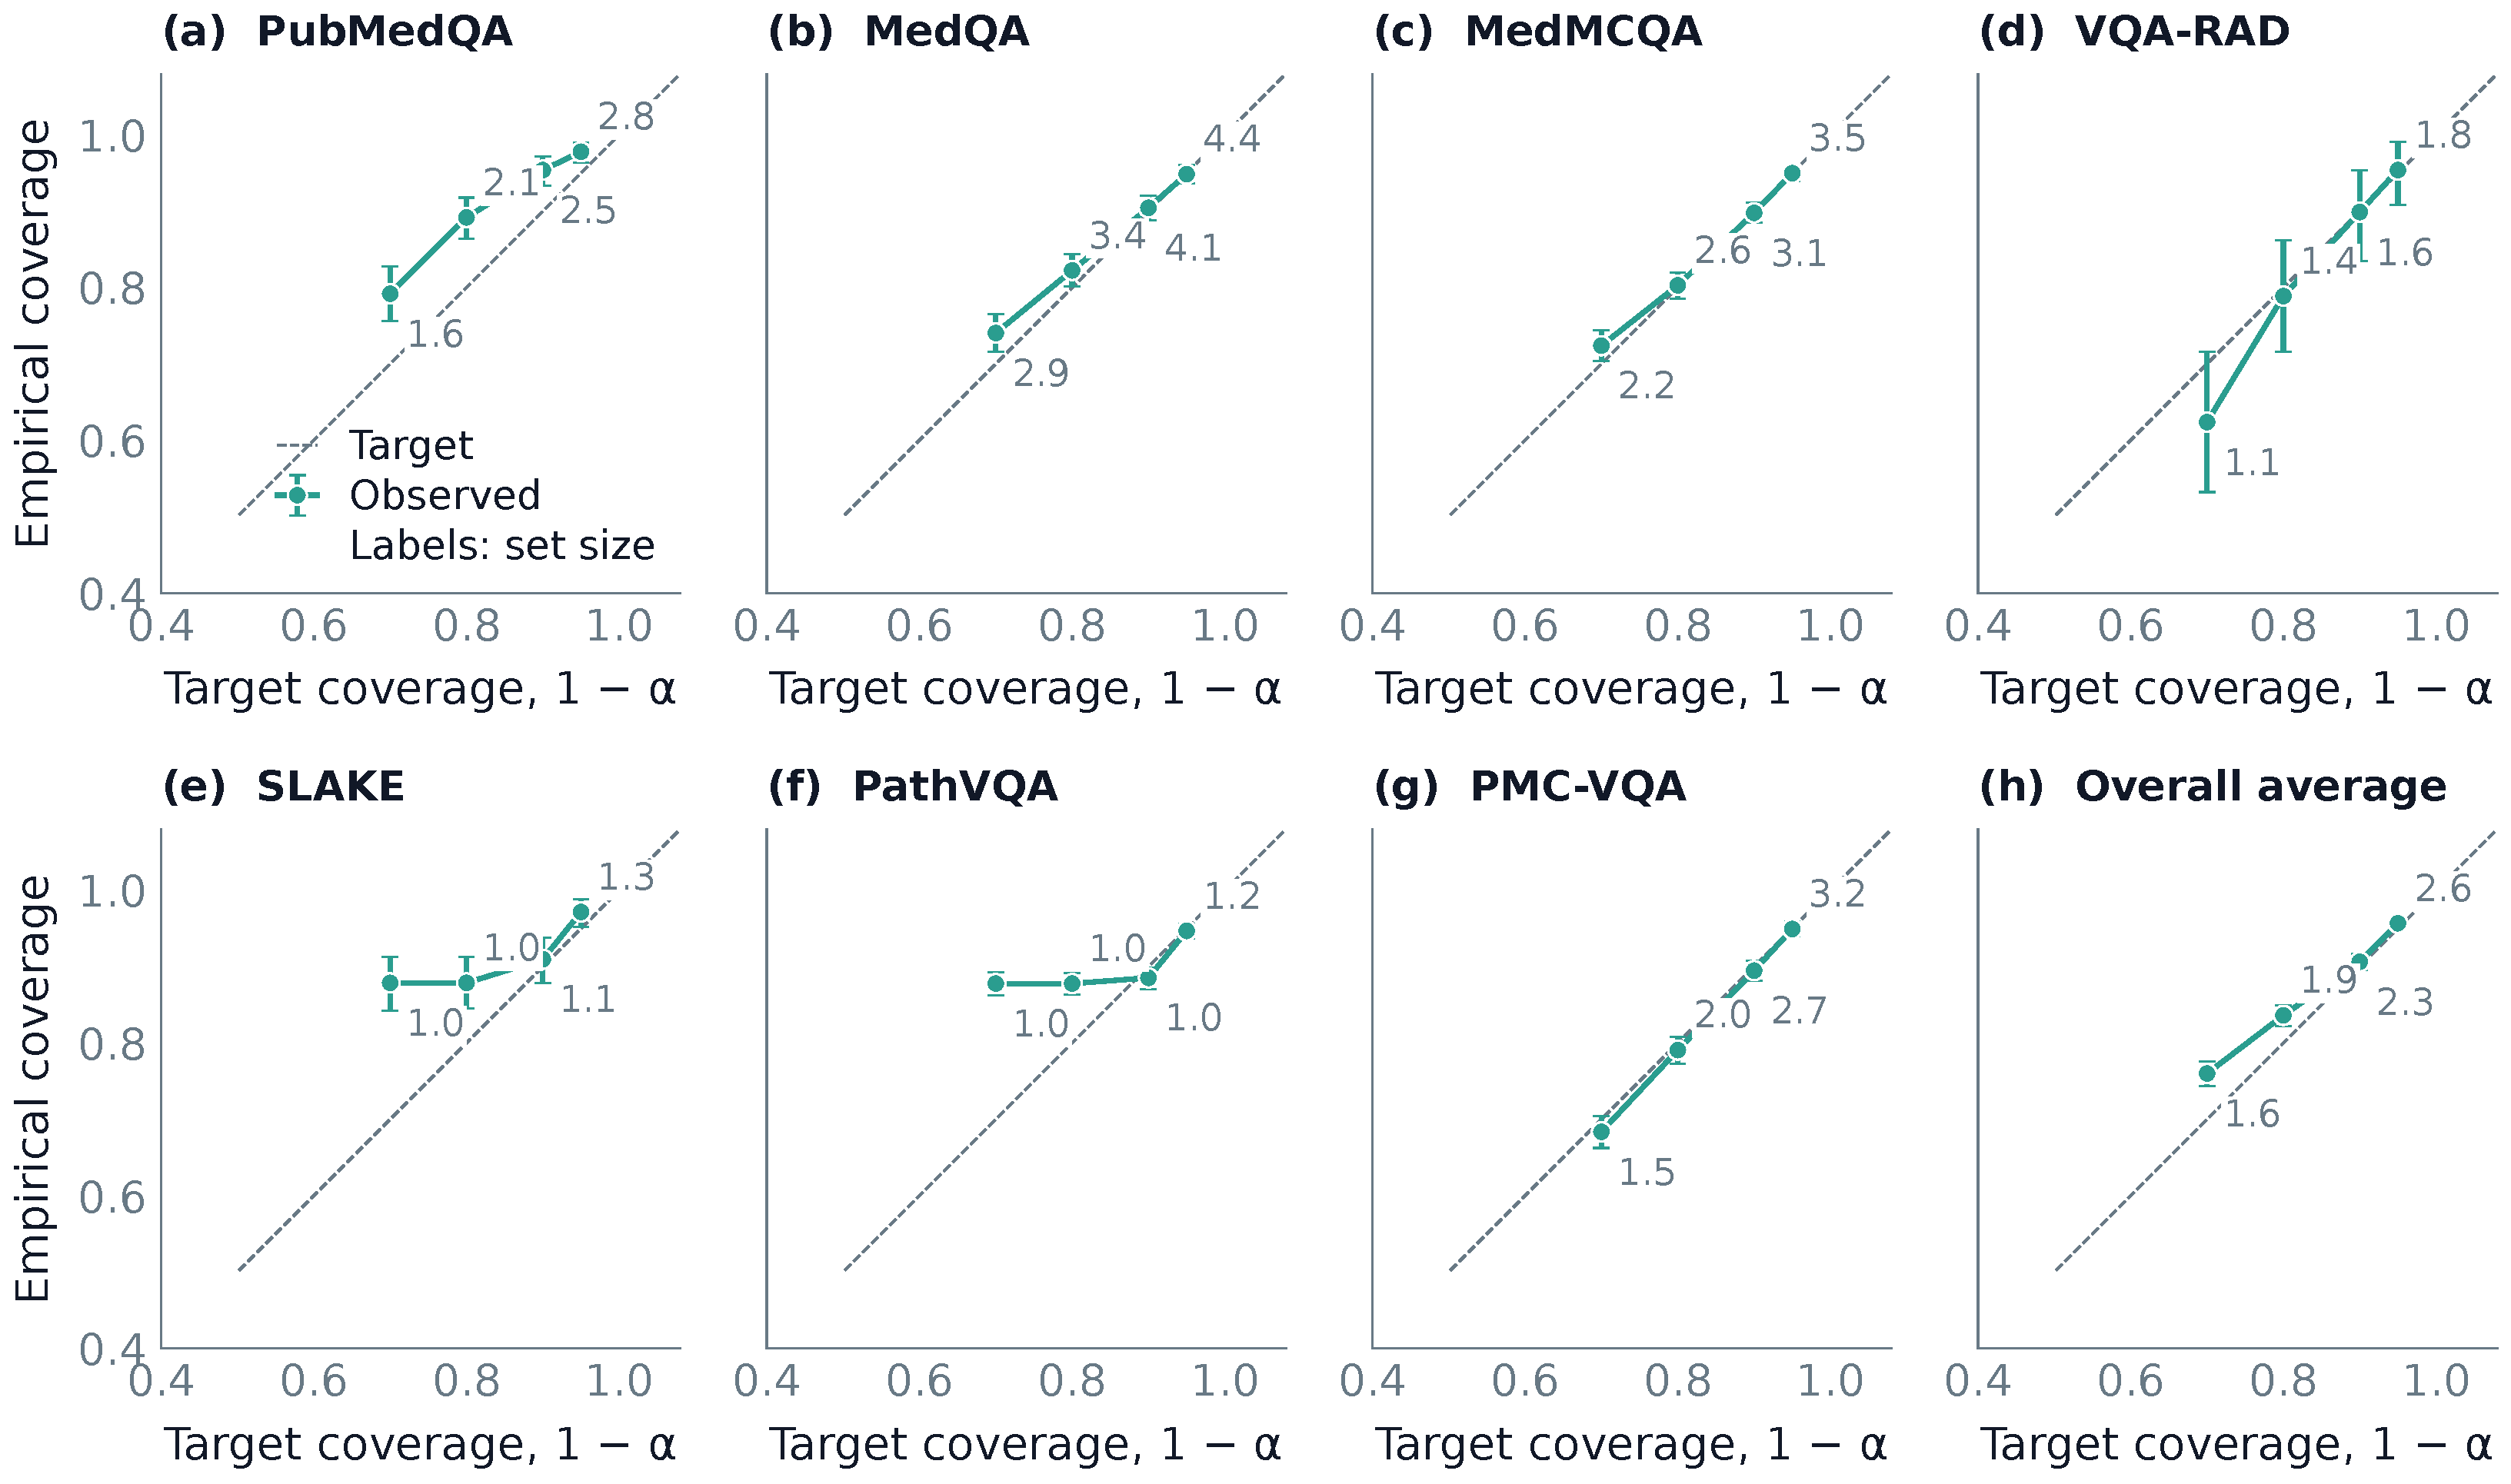
\includegraphics[
        width=\linewidth,
        trim=0 0 0 0,
        clip
    ]{assets/figures/conformal_coverage.pdf}

    \captionof{figure}{
    \textbf{Conformal label coverage.}
    Empirical versus target label coverage; whiskers show 95\%
    bootstrap intervals and annotations report mean prediction-set size.
    }
    \label{fig:conformal_coverage}
\end{minipage}

\end{figure*}

Label coverage is a different objective from singleton accuracy (Fig.~\ref{fig:conformal_coverage}). At a nominal 90\% target, the dataset-balanced NAR-Med analysis attains 90.7\% empirical label coverage with a mean prediction-set size of 2.30. Yet singleton decision coverage varies sharply by task: it is only 3.2\% on MedQA, compared with 98.1\% on PathVQA. MedQA illustrates that a prediction set can contain the correct label at the target rate while remaining too large to yield many accepted decisions; PathVQA illustrates that nearly all examples can yield a singleton even when empirical label coverage is below target. Nominal label coverage, empirical label coverage, and decision coverage therefore answer different questions.

\section{Discussion}
\label{sec:discussion}

The results suggest a staged design perspective for bounded medical assistants. AR-Gen provides a flexible output path when answers must be composed, but AR-LL shows that this flexibility is unnecessary for fixed candidate sets: in our MedGemma comparison, direct label scoring preserves the decision while avoiding most generation latency. When the base decision boundary is inadequate, AR-Head can learn a task-facing interface; AR-Adapt can further change which cases are solved, but its accuracy gain is not uniform and comes with a probability-quality trade-off. NAR-Med occupies a different point in the space: much faster in these implementations, yet sharply dependent on benchmark and modality details. These findings favor choosing the decision computation to match the output contract, not treating one interface as universally superior.

For safety-relevant use, speed is only one part of the value proposition. A candidate distribution supports confidence-based review and conformal sets can distinguish uncertainty about the answer from a singleton decision, but neither guarantees correct or clinically appropriate output. The value of an efficient assistant would come from integrating these signals into a human-reviewed workflow, while auditing whether visual evidence is actually used. Our paired errors, confidence analysis, and image perturbations show why accuracy alone is insufficient to make that judgment. They motivate further evaluation; they do not establish clinical readiness.

\subsection{Limitations}
\label{sec:limitations}
The evaluated AR systems use one backbone family, MedGemma, and NAR-Med is one NAR instantiation. AR/NAR differences also include pretraining, scale, fusion, and optimization; a second AR backbone with the same formulation toggles is needed to test generality. Training uses one seed per run, so paired bootstrap intervals capture test-example sampling uncertainty, not run-to-run variability. Small accuracy differences should therefore not be interpreted as stable across training seeds.

The prepared-data audit groups exact question text and decoded image duplicates, uses known patient/article/group identifiers where available, and quarantines recognized overlaps. It does not audit the pretraining corpora of MedGemma, PubMedBERT, or BiomedCLIP, nor can it rule out unidentified patient overlap or near-duplicates. In addition, MedMCQA and PMC-VQA test partitions are internal holdouts from downloaded training sources, VQA-RAD uses a newly prepared group split, and saved evaluation runs apply a per-dataset cap. These results should not be presented as contamination-free evaluations on the official full test partitions.

AR-LL depends on the renderer's single-token choice labels. Whitespace and case variants are normalized by the evaluator, but multi-token labels, alternative prompt/label conventions, and robustness to these choices were not ablated. The native one-token likelihood baseline should consequently be read as a specified implementation, not a general result for every candidate verbalization. We do not compare against task-specific MCQ competition systems or run label-order and verbalization sensitivity tests. The timing comparison is likewise not a controlled microbenchmark: batch sizes, precision, caching, and timing boundaries vary across systems. We report implementation-level latency, not an architecture-only speedup.

Temperature scaling uses one scalar per trained model, fit on held-out calibration predictions by macro dataset NLL; it is not dataset-specific. We use 15-bin equal-width top-label ECE and do not compare vector scaling, spline calibration, or alternative binning schemes. The primary conformal analysis calibrates the chosen score separately per dataset, while the reference TTA table preserves recorded pooled-quantile operating points. We do not evaluate alternative scores such as normalized margins or representation-based nonconformity, entropy-based abstention, or self-consistency deferral, nor distribution-shift guarantees. Conformal validity requires calibration--test exchangeability and does not guarantee high singleton coverage or accepted accuracy. Finally, missing/shuffled-image tests measure sensitivity to image perturbations, not clinical grounding, and none of these results establish safety or deployment performance.

\section{Conclusion}
\label{sec:conclusion}
Medical SysOne organizes bounded medical decisions around AR-Gen, AR-LL, learned AR interfaces, and NAR-Med. The results separate the latency benefit of removing answer decoding from the predictive effects of learning a head and adapting its representation. Error overlap, confidence, and image perturbations reveal behavior hidden by aggregate accuracy; routing and conformal prediction expose the cost of selective decisions. This formulation-level view offers a basis for building faster, more uncertainty-aware medical assistants, while establishing the evaluation controls and clinical validation still needed before deployment.
